%
% $Id:  ENTER YOUR ID/FILENAME HERE$
%
% This template is based on LLNCS.DEM, the demonstration file of the LaTeX macro 
% package from Springer-Verlag for Lecture Notes in Computer Science, version 2.2 for
% LaTeX2e (see llncs.dem for usage information).
% The template uses the additional definitions based on the master-thesis of Alexander 
% Holupirek (University of Konstanz) and Thomas Zink (University of Konstanz).
% 
% This template was adapted and generalized by Sebastian Kay Belle (University of
% Konstanz) as a generic template for bachelor and master theses (at least for the
% students of the distributed systems laboratory).
%
% Sebastian Kay Belle -- Distributed Systems Laboratory
% Department of Computer and Information Science -- University of Konstanz
% 


% one-sided document style suited for bachelor/master theses (english)
\documentclass[a4paper, twoside]{llncs}
%\usepackage[a4paper,inner=3.5cm,outer=2.5cm,top=2.5cm,bottom=2.5cm,pdftex]{geometry}
%\usepackage[a4paper,inner=3.5cm,outer=2.5cm,pdftex]{geometry}
\usepackage[hmarginratio=3:2,pdftex]{geometry}

%\documentclass[a4paper,twoside]{llncs} 
%\documentclass[12pt,a4paper,twoside,openright]{report}
%\setlength{\oddsidemargin}{-0.4mm} % 25 mm left margin
%\setlength{\evensidemargin}{\oddsidemargin}
%\setlength{\textwidth}{160mm}      % 25 mm right margin
%\setlength{\topmargin}{-5.4mm}     % 20 mm top margin
%\setlength{\headheight}{5mm}
%\setlength{\headsep}{5mm}
%\setlength{\footskip}{10mm}
%\setlength{\textheight}{237mm}     % 20 mm bottom margin
% two-sided document sytel suited for bachelor/master theses (english)
%\documentclass[twoside,a4paper]{llncs} 
% one-sided document sytel suited for bachelor/master theses (german)
%\documentclass[ngerman,a4paper]{llncs} 
% two-sided document sytel suited for bachelor/master theses (german)
%\documentclass[ngerman,twoside,a4paper]{llncs} 

%%%%%%%%%%%%%%%%%%%%%%%%%%%%%%%%%%%%%%%%%%%%%%%%%%%%%%%%%%%%%%%%%%%%%%%%%%%%%%%%%%%%%%%%%%%%%%%%%%%%%%%%%%%%%%%%%
%%% PACKAGES
%%%%%%%%%%%%%%%%%%%%%%%%%%%%%%%%%%%%%%%%%%%%%%%%%%%%%%%%%%%%%%%%%%%%%%%%%%%%%%%%%%%%%%%%%%%%%%%%%%%%%%%%%%%%%%%%%
%\usepackage{tocbibind}
\usepackage{rotating}
\usepackage{ucs}
\usepackage[utf8]{inputenc}
\usepackage{tabularx}
\usepackage[roman]{parnotes}
\usepackage{graphicx}			% graphics, of course
\usepackage{subfigure}
\usepackage{color}                      % to define colors
\usepackage{amsmath, amssymb}		% math symbols for sets etc
\usepackage{multirow}			% for table and tabular, allows multirows and cols
\usepackage[linesnumbered,ruled,vlined,commentsnumbered]{algorithm2e} % extended algorithm package
%\usepackage{ulem}			% for underlining, also changes \em to \underline
					% use \mormalem to undo, however,
					% somehow removes references from toc
\usepackage{fancyvrb}			% fancy verbatim
\usepackage{fancyhdr}                  	% fancy header
\usepackage[colorinlistoftodos]{todonotes} % todo notes
\usepackage{listings}
%\usepackage[font=small,labelfont=bf,tableposition=top]{caption}
\usepackage[all]{hypcap}
\usepackage{hyperref}			% hypertext references, somehow screws up with figures
%\usepackage[svgnames]{xcolor}

%%%%%%%%%%%%%%%%%%%%%%%%%%%%%%%%%%%%%%%%%%%%%%%%%%%%%%%%%%%%%%%%%%%%%%%%%%%%%%%%%%%%%%%%%%%%%%%%%%%%%%%%%%%%%%%%%
%%% SETTINGS
%%%%%%%%%%%%%%%%%%%%%%%%%%%%%%%%%%%%%%%%%%%%%%%%%%%%%%%%%%%%%%%%%%%%%%%%%%%%%%%%%%%%%%%%%%%%%%%%%%%%%%%%%%%%%%%%%
%\DeclareCaptionLabelFormat{andtable}{#1~#2  \&  \tablename~\thetable}

\graphicspath{figures/}			% somehow, doesn't work, thus use command
%\newcommand{\gfx}[0]{../gfx/}
\titlerunning{~}				% set off for llncs	
\authorrunning{~}				% set off for llncs

\newtheorem{thm}{Lemma}%[]             % lemma definition
\newcommand{\factor}[0]{10}

% Listing of algorithms (bug in algorithm2e)
%\renewcommand{\listofalgorithms}{\tocfile{\listalgorithmcfname}{loa}} 

% Bullets for list items
\renewcommand{\labelitemi}{$\bullet$}

% Listings
\lstset{numbers=left, numberstyle=\tiny, stepnumber=1, numbersep=5pt, language=xml, basicstyle=\footnotesize,
 keywordstyle=\color{blue!80!black!100},}

\lstnewenvironment{code}[1][]%
{
   \noindent
   \minipage{\linewidth} 
   \vspace{0.5\baselineskip}
   \lstset{basicstyle=\ttfamily\footnotesize,frame=single,#1}}
{\endminipage}

%%%%%%%%%%%%%%%%%%%%%%%%%%%%%%%%%%%%%%%%%%%%%%%%%%%%%%%%%%%%%%%%%%%%%%%%%%%%%%%%%%%%%%%%%%%%%%%%%%%%%%%%%%%%%%%%%
%%% SETTINGS FOR THE HYPERREF PACKAGE
%%%%%%%%%%%%%%%%%%%%%%%%%%%%%%%%%%%%%%%%%%%%%%%%%%%%%%%%%%%%%%%%%%%%%%%%%%%%%%%%%%%%%%%%%%%%%%%%%%%%%%%%%%%%%%%%%
\definecolor{internal-link}{rgb}{0.2, 0.26, 0.43}
\definecolor{cite-link}{rgb}{0.4, 0.61, 0.46}
\definecolor{url-link}{rgb}{0.4, 0.46, 0.63}

\hypersetup{
  colorlinks=true,
  linkcolor=internal-link,
  citecolor=cite-link,
  urlcolor=url-link
}

%%%%%%%%%%%%%%%%%%%%%%%%%%%%%%%%%%%%%%%%%%%%%%%%%%%%%%%%%%%%%%%%%%%%%%%%%%%%%%%%%%%%%%%%%%%%%%%%%%%%%%%%%%%%%%%%%
%%% KW SETTINGS FOR ALGORITHMS2E (see algorithm2e documentation for details)
%%%%%%%%%%%%%%%%%%%%%%%%%%%%%%%%%%%%%%%%%%%%%%%%%%%%%%%%%%%%%%%%%%%%%%%%%%%%%%%%%%%%%%%%%%%%%%%%%%%%%%%%%%%%%%%%%
% define your language keywords here (e.g. \SetKw{To}{to})
%\SetKw{To}{to}
%\SetKw{Not}{not}
% define your data keywords here (e.g. \SetKwData{Counters}{counters})
% define your function keywords here (e.g. \SetKwFunction{Compress}{Compress})

%%%%%%%%%%%%%%%%%%%%%%%%%%%%%%%%%%%%%%%%%%%%%%%%%%%%%%%%%%%%%%%%%%%%%%%%%%%%%%%%%%%%%%%%%%%%%%%%%%%%%%%%%%%%%%%%%
%%% HEADER/FOOTER (see the fancyhdr documentation for details)
%%%%%%%%%%%%%%%%%%%%%%%%%%%%%%%%%%%%%%%%%%%%%%%%%%%%%%%%%%%%%%%%%%%%%%%%%%%%%%%%%%%%%%%%%%%%%%%%%%%%%%%%%%%%%%%%%
\setlength{\headheight}{15pt}
 
\pagestyle{fancy}
\renewcommand{\chaptermark}[1]{\markboth{#1}{}}
\renewcommand{\sectionmark}[1]{\markright{#1}{}}
\renewcommand{\headrulewidth}{0.5pt}
\renewcommand{\footrulewidth}{0.5pt}
 
\fancyhf{}
\fancyhead[LE,RO]{\thepage}
\fancyhead[RE,LO]{\textit{\nouppercase{\rightmark}}}
\fancyfoot[EL,OR]{\thepage}
%\fancyhead[LE,LO]{\thepage}
%\fancyhead[RE,RO]{\textit{\nouppercase{\rightmark}}}
%\fancyfoot[EL,OL]{\thepage}

\fancypagestyle{plain}{ %
\fancyhf{} % remove everything
\renewcommand{\headrulewidth}{0pt} % remove lines as well
\renewcommand{\footrulewidth}{0pt}}

%%%%%%%%%%%%%%%%%%%%%%%%%%%%%%%%%%%%%%%%%%%%%%%%%%%%%%%%%%%%%%%%%%%%%%%%%%%%%%%%%%%%%%%%%%%%%%%%%%%%%%%%%%%%%%%%%
%%% OTHER DEFINITIONS
%%%%%%%%%%%%%%%%%%%%%%%%%%%%%%%%%%%%%%%%%%%%%%%%%%%%%%%%%%%%%%%%%%%%%%%%%%%%%%%%%%%%%%%%%%%%%%%%%%%%%%%%%%%%%%%%%
\def\dotuline{\bgroup
  \ifdim\ULdepth=\maxdimen  % Set depth based on font, if not set already
   \settodepth\ULdepth{(j}\advance\ULdepth.4pt\fi
  \markoverwith{\begingroup
  \advance\ULdepth0.08ex
  \lower\ULdepth\hbox{\kern.15em .\kern.1em}%
  \endgroup}\ULon}

\def\dashuline{\bgroup
  \ifdim\ULdepth=\maxdimen  % Set depth based on font, if not set already
   \settodepth\ULdepth{(j}\advance\ULdepth.4pt\fi
  \markoverwith{\kern.15em
  \vtop{\kern\ULdepth \hrule width .3em}%
  \kern.15em}\ULon}

% --- verbatim environments
%\VerbatimFootnotes 
\DefineVerbatimEnvironment{xml}{Verbatim}
{
% gobble=2,
  frame=single,% framerule=0.25pt,
% xleftmargin=1em, xrightmargin=1em,
  fontfamily=courier, fontsize=\scriptsize,
  commandchars=\\\{\}
}
\DefineVerbatimEnvironment{fs}{Verbatim}
{
% gobble=2,
  frame=lines, framesep=3mm,
  labelposition=topline,
  fontfamily=courier, fontsize=\footnotesize,
  commandchars=\\\{\}
}
\DefineVerbatimEnvironment{xquery}{Verbatim}
{
% gobble=2,
  frame=lines, framesep=3mm,
  labelposition=topline,
  %framerule=0.4pt, % default 0.4pt
  fontfamily=courier, fontsize=\footnotesize,
  commandchars=\\\{\}
}

% Definition environment
\newtheorem{mydef}{Definition}

%%%%%%%%%%%%%%%%%%%%%%%%%%%%%%%%%%%%%%%%%%%%%%%%%%%%%%%%%%%%%%%%%%%%%%%%%%%%%%%%%%%%%%%%%%%%%%%%%%%%%%%%%%%%%%%%%
%%% DOCUMENT
%%%%%%%%%%%%%%%%%%%%%%%%%%%%%%%%%%%%%%%%%%%%%%%%%%%%%%%%%%%%%%%%%%%%%%%%%%%%%%%%%%%%%%%%%%%%%%%%%%%%%%%%%%%%%%%%%
\begin{document}

%%%%%%%%%%%%%%%%%%%%%%%%%%%%%%%%%%%%%%%%%%%%%%%%%%%%%%%%%%%%%%%%%%%%%%%%%%%%%%%%%%%%%%%%%%%%%%%%%%%%%%%%%%%%%%%%%
%%% TITLE PAGE -- CHOOSE THE APPROPRIATE TITLE PAGE HERE (AND MODIFY THEM TO YOUR LIKING)
%%%%%%%%%%%%%%%%%%%%%%%%%%%%%%%%%%%%%%%%%%%%%%%%%%%%%%%%%%%%%%%%%%%%%%%%%%%%%%%%%%%%%%%%%%%%%%%%%%%%%%%%%%%%%%%%%
\pagenumbering{alph}
\pagestyle{empty}
%\pagestyle{plain}
%\input{titlepage_std_en} % include your titlepage here (standard title page)
%\input{titlepage_std-signet_en} % include your titlepage here (standard title page with university signet)
\begin{titlepage}
\begin{minipage}{0.9\linewidth}
\end{minipage}
%\vfill
%\begin{center}
%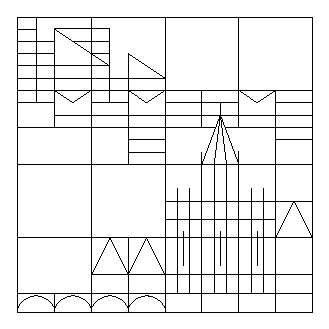
\includegraphics[scale=1]{figures/signet} % signet U KN
%\end{center}
\vspace{7mm}
%\vfill
{\sf
\begin{center}
{\Large University of Konstanz} \\
\vspace{2mm}{\Large Department of Computer and Information Science} \\ 
\vspace{4mm}
\rule{0.98\linewidth}{2pt}\\
\vspace{4mm} 
{\huge {\bf {\sffamily{Master Thesis}}}}\\
\vspace{10mm}
{\huge A Visual Analytics Approach for Comparing Tree-Structures.}\\
\vspace{10mm}
{\em {\sffamily{in fulfillment of the requirements to achieve the degree of \\ 
\vspace{2mm} {\bf \sffamily{Master of Science (M.Sc.)}}}}}\\
\vspace{2mm}
\rule{0.98\linewidth}{2pt}\\
\vspace{6mm}{\Large \bf \sffamily{Johannes Lichtenberger}}\\
\vspace{0mm}{Matriculation Number :: 01/584875}\\
\vspace{0mm}{E-Mail :: $\langle$firstname$\rangle$.$\langle$lastname$\rangle$@uni-konstanz.de}\\
\vspace{6mm}
{\small
\begin{tabular}{l  p{5mm}  r}
{\bf {\sffamily{Field of Study}}} ::  Information Engineering & & {\bf \sffamily{First Assessor}} ::  {\em Prof. Dr. M. Waldvogel}\\
{\bf {\sffamily{Focus}}} :: {\em Informatik der Systeme} & & {\bf \sffamily{Second Assessor}} ::  {\em Jun.-Prof. Dr. Tobias Schreck}\\
{\bf {\sffamily{Group}}} :: {\em Distributed Systems Group} & & {\bf \sffamily{Advisor}} ::  {\em M.Sc. Sebastian Graf}\\
\end{tabular}\\
}
\end{center}
}
\vfill
\end{titlepage}




 % include your titlepage here (unconventional title page with university signet above 
%\input{titlepage_fancy-teaser_en} % include your titlepage here (unconventional title page with space for a teaser image)
%\pagestyle{fancy}
\cleardoublepage

%%%%%%%%%%%%%%%%%%%%%%%%%%%%%%%%%%%%%%%%%%%%%%%%%%%%%%%%%%%%%%%%%%%%%%%%%%%%%%%%%%%%%%%%%%%%%%%%%%%%%%%%%%%%%%%%%
%%% PREAMBLE
%%%%%%%%%%%%%%%%%%%%%%%%%%%%%%%%%%%%%%%%%%%%%%%%%%%%%%%%%%%%%%%%%%%%%%%%%%%%%%%%%%%%%%%%%%%%%%%%%%%%%%%%%%%%%%%%%
\newpage
\pagestyle{fancy}
%\voffset=10mm % optical enhancement!!!
\pagenumbering{roman} % set the page numbering style to roman numbers
\cleardoublepage
\thispagestyle{empty}
\vspace*{0.5\textheight}
\begin{center}
dedicated to...
\end{center}
\newpage
 % refer your preamble here
\clearpage

%%%%%%%%%%%%%%%%%%%%%%%%%%%%%%%%%%%%%%%%%%%%%%%%%%%%%%%%%%%%%%%%%%%%%%%%%%%%%%%%%%%%%%%%%%%%%%%%%%%%%%%%%%%%%%%%%
%%% ACKNOWLEDGEMENTS
%%%%%%%%%%%%%%%%%%%%%%%%%%%%%%%%%%%%%%%%%%%%%%%%%%%%%%%%%%%%%%%%%%%%%%%%%%%%%%%%%%%%%%%%%%%%%%%%%%%%%%%%%%%%%%%%%
\newpage
%\setcounter{page}{1}
\input{acknowledgements} % refer your acknowledgments here
%\addcontentsline{toc}{section}{Acknowledgments}

%%%%%%%%%%%%%%%%%%%%%%%%%%%%%%%%%%%%%%%%%%%%%%%%%%%%%%%%%%%%%%%%%%%%%%%%%%%%%%%%%%%%%%%%%%%%%%%%%%%%%%%%%%%%%%%%%
%%% ABSTRACT
%%%%%%%%%%%%%%%%%%%%%%%%%%%%%%%%%%%%%%%%%%%%%%%%%%%%%%%%%%%%%%%%%%%%%%%%%%%%%%%%%%%%%%%%%%%%%%%%%%%%%%%%%%%%%%%%%
\newpage
\setcounter{page}{1}
\input{abstract} % refer your abstract here
\addcontentsline{toc}{section}{\abstractname}
\cleardoublepage

%%%%%%%%%%%%%%%%%%%%%%%%%%%%%%%%%%%%%%%%%%%%%%%%%%%%%%%%%%%%%%%%%%%%%%%%%%%%%%%%%%%%%%%%%%%%%%%%%%%%%%%%%%%%%%%%%
%%% TABLE OF CONTENT, LIST OF FIGURES & LIST OF TABLES
%%%%%%%%%%%%%%%%%%%%%%%%%%%%%%%%%%%%%%%%%%%%%%%%%%%%%%%%%%%%%%%%%%%%%%%%%%%%%%%%%%%%%%%%%%%%%%%%%%%%%%%%%%%%%%%%%
\newpage
\pagestyle{fancy}
\setcounter{tocdepth}{2}
\tableofcontents
\newpage
\pagestyle{fancy}
\addcontentsline{toc}{section}{\listfigurename}
\listoffigures
\newpage
\pagestyle{fancy}
\addcontentsline{toc}{section}{\listtablename}
\listoftables
\cleardoublepage
%\addcontentsline{toc}{section}{\listtodoname}

%%%%%%%%%%%%%%%%%%%%%%%%%%%%%%%%%%%%%%%%%%%%%%%%%%%%%%%%%%%%%%%%%%%%%%%%%%%%%%%%%%%%%%%%%%%%%%%%%%%%%%%%%%%%%%%%%
%%% SECTIONS
%%%%%%%%%%%%%%%%%%%%%%%%%%%%%%%%%%%%%%%%%%%%%%%%%%%%%%%%%%%%%%%%%%%%%%%%%%%%%%%%%%%%%%%%%%%%%%%%%%%%%%%%%%%%%%%%%
\pagestyle{fancy}
\pagenumbering{arabic} % set the page numbering to arabic page numbers
\setcounter{page}{1}
\input{introduction} % refer your introduction here
\cleardoublepage
\section{Preliminaries and State-of-the-Art}\label{sec::relwork} %Analysis \& visualization of differences in tree-structured data}\label{sec::hierarichaldata}

\subsection{Introduction}
Today's storage capabilities facilitate the growing amount of data which is most often collected and stored without filtering or preprocessing.
One of the consequences is the information overload problem defined as:

\begin{itemize}
\item Irrelevant to the current task at hand.
\item Processed or presented in an inappropriate way.
\end{itemize}

To turn these issues into advantages the science called "Visual Analytics" recently became popular. 

James J. Thomas and Kristin A. Cook coined the term "Visual Analytics" in \cite{VISUAL_ANALYTICS} and defined it as: "Visual analytics is the science of analytical reasoning facilitated by interactive visual interfaces." It combines (semi-)automatic analytical analysis with interatice visualization techniques, thus emphasizes both cognitive human and electronical data processing strenghts.

Whereas the information seeking mantra is described as "overview first, zoom/filter, details on demand" Keim et al defined the Visual Analytics mantra as:

"Analyse First -
Show the Important -
Zoom, Filter and Analyse Further -
Details on Demand" \cite{keim2008visual}

This implies and confirms the important role of humans in the analysis process. As meantioned in the introduction humans are trained to interpret visual impressions but often fail in the same way to construe inappropriate representations as for instance the tabular representation of mathematical functions with lots of numbers specifying the input $x$ and the result $f(x)$). Therefore it is inevitable to assess analysts by interactive visualizations.

The Visual Analytics process proposed by Keim et al. is depicted in Fig. \ref{fig:visualanalyticsprocess}.

\begin{figure}[htb]
\center{\includegraphics[width=\textwidth - 6em]
{figures/visualanalyticsprocess}}
\caption{\label{fig:visualanalyticsprocess} Visual Analytics Process proposed by Keim et al. Presented in \cite{keim2008visual}.}
\end{figure}

Our Visual Analytics pipline is largely influenced by this process. Chapter \ref{sec::differences} describes the addition of new edit-operations in Treetank and two types of diff-algorithms. These fundamental to analytical reasoning and therefore denote Data Mining methods in Fig. \ref{fig:visualanalyticsprocess}. Models underlying the different views are built based on the output of the the difference-algorithms and thus represent directly the model entity in Fig. \ref{fig:visualanalyticsprocess}. Visualizations (Chapter \ref{sec::visualizations} receive user input and build models through invocation of an ID-based diff algorithm. Parameter changes in the GUI of our main visualization, a Sunburst view tailored to tree-structure comparisons, influence and change the models and in turn change the visualizations according to their output. However user interaction might change visualization(s) without having any impact on the model(s).

Comparing tree-structures by a Visual Analytics approach requires analytical reasoning through the computation of differences in the first place. Thus the next section describes existing ID-less algoritms focused on XML-comparison. A short study and summary of existing visualization techniques follows.

\subsection{Analysis of differences}
Line by line textual diffs are based on algorithms which solve the Longest Common Subsequence (LCS) problem. Whereas they are sufficient to track changes in flat text-files, tree-structures need more sophisticated methods as pointed out in the introduction.

The \emph{Extendable Markup Language} (XML) is a textual data format for encoding and structuring documents in machine- and human-readable form. Its inherent data structure is a rooted, ordered, labeled tree. 

\begin{mydef}
A rooted \textbf{tree-structure} is an acyclic connected graph, which starts with a root node whereas every node has zero or more children with the exception of the root-node having exactly one parent-node. We define a tree T as $T = (N, E, root(T))$ whereas N denotes all nodes, E denotes edges, the relation between child- and parent-nodes whereas each child except the root-node has exactly one parent node, root(T) defines a root-node which is the only node having no parent.
\end{mydef}

\begin{mydef}
A rooted, ordered, labeled tree is a tree-structure which extends the rooted tree-definition by defining a specific order for child nodes (that is extending the parent/child edge relation E) and a label for each node. Furthermore each node has a label. Thus T is an ordered, labeled, tree if $T = (N, E, root(T), \Lambda(n) \in \Sigma)$. $\Sigma$ is a finite alphabet and $n$ is a node in the tree.
\end{mydef}

Thus a tree is more restricted than a hierarchy based on a directed acyclic graph (DAG) in which every node except the root\footnote{which has no parent} might have one or more parent nodes.

Many algorithms have been developed to determine differences in tree-structures for instance to provide deltas, which represent a compact version of the changes to the original document.

Next, some essential terms are defined to set the stage for the upcoming sections.

The tree-to-tree correction problem tries to transform a source tree into a destination tree by edit-operations. 

\begin{mydef}
An edit-operation is an atomar operation which changes a tree.
\end{mydef}

Deltas are defined as:

\begin{mydef}
A directed delta/edit script is a sequence or set of (elementary) edit-operations which when applied to one version v1, yields another version v2.
\end{mydef}

\begin{mydef}
A symmetric delta is a directed delta which is invertible.
\end{mydef}

In the following we use the term \emph{delta} and \emph{edit script} interchangeably in the generic form meaning directed delta. Each edit operation is usually defined with a fixed cost (usually unit cost).

\begin{mydef}
A minimal edit script is a minimum cost edit script.
\end{mydef}

Besides providing a minimal or close to minimal edit script further metrics of a diff-algorithm are the CPU runtime and the compactness of the delta in terms of storage-space (e.g. it is in most cases sufficient to define edit operations on subtrees, such as a delete- or move-operation which usually removes the whole subtree).

Some of the most popular approaches to detect differences in XML-documents and to generate a delta are described next.

\subsubsection{DeltaXML\cite{DELTAXML}}
uses attributes in the deltaxml namespace to specify changes. For instance \texttt{deltaxml:deltaV2="A!=B"} specifies that the element containing this attribute has been changed from revision A to revision B. Nodes which exist in revision A but not in revision B are marked with \texttt{deltaxml:deltaV2="A"} and vice versa. Due to this, the deltas generated by DeltaXML are invertible. Elements are matched according to element types, the level in the tree and the Longest Common Sequence (LCS). Furthermore matching PCDATA nodes may optionally be prefered. Similar, attribute-IDs in the deltaxml-namespace may be used to mark nodes with unique IDs. Marking all nodes with an ID generates a minimum edit distance delta file.

\subsubsection{XyDiff\cite{cobena2002detecting}}
has been developed in the context of Xyleme, an XML database warehouse. Initially a unique persistent identifier XID is assigned to each node. XID-Maps are generated through a postorder traversal whereas initially integers from 1 to n are assigned. N denotes the number of nodes in the original tree. Added nodes in the revision to compare are assigned further integers starting from n + 1 again by a postorder traversal. Nodes which are not present in the new revision are removed resulting in gaps. Assuming an initial range of identifiers from (1-474) it might result in several ranges, for instance (1-13),(17-447),(450-474) which means that the nodes with the XIDs 14, 15 and 16 have been deleted as well as the nodes 448 and 449. The algorithm for the actual change detection is outlined in the next paragraph. Inserts, Deletes, Updates and Moves are supported.

First nodes with ID attributes defined in a DTD are matched. Then signatures are generated in a bottom-up traversal, which are hash values computed from the value of the current node and all child signatures. Furthermore weights are computed and defined as the text node sizes which are summed up for each child node. A priority queue is build, whereas the largest weights of the new document are prioritised. The largest subtrees are considered first to be matched based on their signatures. If more than one node has the same signature a heuristic is used, otherwise the child nodes are added to the queue. Whenever nodes match each subtree and anchestor pair is going to be matched as long as the labels are equal. The propagation to anchestor nodes depends on the node weight. A heuristic is used to substitute the computation of largest order preserving common subsequences for the move-operation. As heuristics are used the resulting edit-scripts/deltas are not guaranteed to be minimal.

The CPU runtime of the algorithm is $O(n \log n)$.

\subsubsection{LaDiff / Fast Match Simple Editscript (FMSE)\cite{chawathe1996change}}\label{subsec::ladiff}
operates on different versions of LaTeX documents. It has been developed to demonstrate and measure the feasability of an approach to detect changes in hierarichally structured information.

Chawathe et al. divides this task into two main problems:

\begin{description}
\item[the Good Matching problem] is the problem of finding matches between the two trees, which are either equal for some predefined function or approximately equal.
\item[finding a Minimum Conforming Edit Script (MCES)] is the second obstacle. An \emph{edit script} is a sequence of edit operations wh the source file which transform it into the target document once applied. Costs are therefore applied to every edit operation.
\end{description}

The algorithms used to solve these two problems operate on rooted, ordered, labeled trees. Four edit operations (\texttt{insert}, \texttt{delete}, \texttt{update} and \texttt{move} are defined with unit costs.

The algorithm proves to yield minimum edit scripts in case the assumption holds true that no more than one leaf node is considered equal to a predefined function which compares the values of leaf nodes and the labels match. XML does provide labels in the form of \texttt{QName}s for \texttt{element}- and \texttt{attribute}-nodes and a slightly restricted alphabet for \texttt{text}-nodes. Thus either text-node values have to be compared or \texttt{QName}s.

Thus the first criterium for leaf nodes is 

\begin{equation} 
compare(v(x), v(y)) \leq f\ such\ that\ 0 \leq f \leq 1
\end{equation}

Inner nodes are match candidates according to the forumla 

\begin{equation}
\frac{|common(x, y)|}{max(|x|,|y|)} > t\ and\ label(x) = label(y)
\end{equation}

$common(x,y) = \{(w,z) \in M | x\ contains\ w\ and\ y\ contains\ z\}$ whereas a \begin{quote}node x contains a node y if y is a leaf node descendant of x and $|x|$ denotes the number of leaf nodes x contains.\end{quote} The threshold t is defined as $0.5 \leq t \leq 1.0$.

In a first step the good matching problem is solved by means of concatenating nodes/labels starting from bottom up and finding a LCS at each level of the tree. Furthermore if nodes are left which are equal according to the predefined function they are subsequently matched on each level. If the assumption does not hold which might be the case for several XML-documents, especially in data centric XML files the algorithm yields large output-deltas according to Lindholm et al.\cite{lindholm2006fast} and R"onnau et al.\cite{ronnau2009efficient}. This is a direct result of the ambigiouty of the LCS as well as of the subsequent matching of nodes on every level. However this is a problem common to almost all differencing algorithms and can be minimized by proper definitions of the similarity functions for leaf- and innder-nodes.

After that in a breadth first traversal nodes are inserted, updated, moved and deleted. The children of each node are aligned based on the LCS once again. Nodes which are matched but not in the LCS are moved. The order in which operations are applied to the source tree and the edit script is crucial to the correctness of the algorithm.

It is apparent that a large number of moves are appended to edit scripts in case the assumption that every leaf node in the old revision is similar to at most one leaf node in the old revision. If this assumption does not hold true the algorithm yields suboptimal deltas due to mismatches. A postprocessing step reduces other mismatches and thus move-operations such that children of matched nodes, which have not the same parent are tried to match with children of the same parent in the other tree, thus correcting some misaligned nodes. Note that this step can not reduce errors propagating from mismatched leaf nodes up in the tree.

The time complexity is $O(n*e+e^2)$.

\subsubsection{X-Diff\cite{wang2003x}}
operates on unordered, labeled trees. No matter how the order among child-nodes changes it lacks semantic difference and therefore is considered to be equal. 

First XHash values are computed in a bottom up postorder traversal for every node which represent the entire subtree rooted at the respective node.
The hash computation does not include the child order, such that isomporhic trees can be matched in subsequent steps.

Next the trees are traversed starting from the root-nodes. Nodes on currentLevel+1 are filtered out which have equal hash values.

Signatures defined as $Signature(x) = /name(x_{1})/.../name(x_{n})/name(x)/type(x)$ for element nodes and $Signature(x) = /name(x_{1})/.../name(x_{n})/type(x)$ for text nodes are used to determine if nodes are considered to match. Note that in case of a text node it does not contain the value in the signature. This decision leads to the support of update-Operations, which are only defined as an edit cost for text nodes. 

Initially leaf nodes are compared based on a predefined edit distance function and a matching/distance-value tuple is stored in a table. To compute the edit distance between subtrees the minimum-cost maximum flow algorithm \cite{zhang1996constrained} is used.

Based on a minimum cost matching and the distance table an edit script can be computed.

The runtime has been considered for each of the three steps separately: 

\begin{enumerate}
\item {\bf{Parsing and Hashing}}: $O(|T_{1}| + |T_{2}|)$
\item {\bf{Mapping}}: $O(|T_{1}| \times |T_{2}|) \times max\{deg(T_{1}, deg(T_{2})\} \times \log_{2}(max\{deg(T_{1}), deg(T_{2})\}))$
\item {\bf{Generating Minimum-Cost Edit Script}}: $O(|T_{1}| + |T_{2}|)$
\end{enumerate}

\subsubsection{DocTreeDiff\cite{ronnau2009efficient}}
is designed for difference detection in document-centric XML documents. XML documents come in two-flavors. Document-centric XML documents are usually written by an author such as website-content or a DocBook-based article whereas data-centric documents are usually automatically created. Leaf nodes in document-centric XML usually can be descriminated very well.

It is stated that document-centric XML typically is restricted in depth by a document format through a Schema or DTD but the width, which grows with increasing text length, is not. Furthermore almost all content is stored in the leafes whereas internal nodes represent the structure of the document (sections, paragraphs, lists, descriptions...). Based on this observation R\"onnau et al. state the following assumptions

\begin{enumerate}
\item Content is stored within the leaves.
\item Changes to structure and markup will be performed on a higher level within the tree.
\item Many non-leaf nodes are equal due to identical markup.
\end{enumerate}

Based on these assumptions the algorithm relies heavily on the computation of a LCS on leaf nodes.

\begin{enumerate}
\item First the algorithm computes the LCS on leaf nodes based on their hash values and the depth in the tree.
\item Next, a bottom up traversal of all leaf nodes which are considered equal follows to detect updates for each anchestor node. All nodes are marked which have been processed to skip the process for subsequent bottom-up traversals when an anchestor node is the same.
\item Last, deletes, inserts and moves are detected. A second bottum up traversal starting at leaf nodes which have not matched, detects nodes which are in the old revision but not in the new are considered as being deleted. At every level the child nodes of the parents are searched for the neares node which has been marked as matched during the LCS computation. If one is found the traversal stops. The same holds for inserted nodes if the reverse condition is true. Therefore the bottom-up traversal detects the largest possible subtrees to delete or insert, since the edit operations are not defined on single nodes. Furthermore adjacent deletions or insertions are glued together. Delete/insert-operations on the same subtrees are combined into one move-Operation.
\end{enumerate}

Thus it does not detect moves if internal nodes are inserted but large subtrees have not changed. The runtime complexity is $O(leaves(T)D + n)$ whereas $T$ is the sum of nodes in both trees and $D$ is the number of edit operations. The space complexity is $O(T+D)$.

\subsubsection{Faxma\cite{lindholm2006fast}}
uses fast sequence aligning. First the input documents are parsed into XAS tokens, which preserves the XML structure. They support three edit operations: \texttt{insert}, \texttt{delete} and \texttt{move} since they claim that subtrees are often moved. Updates are nontheless handled through the combination of \texttt{delete/insert} pairs which is similar to the approach used by \emph{DocTreeDiff}. Based on \emph{rolling-hashes} a sliding window iterates over sequences derived from transforming both XML documents. A rolling-hash can be updated really fast if the right hash-function is chosen. If so, only the old value, the new value and the previous hash-value is needed \cite{RollingHash}:

\begin{equation}
h(S_{i+1}) = H(h(S_{i}), s_{i} , s_{i+n+1})
\end{equation}

To quickly find maximum length matches, window sizes of length $S = <48,32,16,8,4,2,1>$ are used.

At first all nodes are marked as $ins(node)$ in both sequences. Starting with the greatest size, matches are searched for in a zigzag-pattern, whereas matched sequences are extended alternately moving forward and backward until no further matches are found. These matches are marked with\\ $cpy([start\ index], [end\ index])$ in the sequence of the updated document. Any matching sequences are then removed from the sequence representing the old revision, finally resulting in the configuration, that only deleted nodes are left in this sequence.

Since the matches are not necessarily aligned on subtree boundaries the match-list must be transformed back into the tree-domain.

The algorithm serializes match lists in a sequential traversal, providing the \texttt{start-} and \texttt{end-tag} has been encountered. A queue of tentative node- and tree-reference tags is maintained to either discard changes partially or serialize the results. Details of this algorithm are omitted, since the resulting delta does not fit our purpose. The delta is a script which includes identifiers to matched nodes with inserted sequences between. It is thus not defined in terms of an edit script and thus not directly useful for our purpose.

\subsubsection{Summary}
The problem in common to all approaches is to efficiently compute a minimum or near minimum edit script to transform the first into the second tree. Unfortunately a guaranteed minimum edit script for the the tree-to-tree correction problem is known to be bound in the runtim by \\$O(nm\ min(depth(T1), leaves(T1))\ min(depth(T2),\ leaves(T2)))$, with $n$, $m$ denoting the number of nodes of the trees $T1$ , $T2$. Using heuristics speeds up the process but it does in most cases produce non optimal (minimal) edit scripts which might be counterintuitive to humans, because of mismatched nodes which have not been changed. Every diff-algorithm has its strength and pitfalls. Depending on the input and expected modification patterns some algorithms provide better results than others. All algorithms work best if leaf nodes can be descriminated very well. Comparing document oriented XML thus usually procudes better results in comparison to data centric XML in terms of minimum or near minimum edit-scripts/deltas.

Memory consumption is very important considering larger XML instances ranging from 1Gb and far above. Reducing the cost of computing the LCS which has a large memory footprint might be mandatory but also results in heuristics. A survey of the wide range of algorithms is summarized in \cite{cobena2002comparative}. Several algorithms are described and compared according to the attributes memory consumption, time complexity supported operations and ordered/unordered. Ordered/unordered denotes if anchestor/child relationships and the child order is considered (ordered) or not (unordered). 

In summary a trade-off between the minimality of edit scripts/operations and the memory consumption as well as the time complexity of the algorithm exists. Furthermore no algorithm exists which outperforms and in respect to the edit-script cost produces always better results than the others while comparing trees of different domains and characteristics. It heavily depends on the change pattern of the input document.

\begin{table}[tb]
\centering 
\begin{tabular}[r]{|l|c|c|c|c|} 
\hline
& \textbf{runtime comp.} & \textbf{space comp.} & \textbf{tree model} & \textbf{move support}\\
\hline
\hline
\textbf{DeltaXML} & not published & not published & not published & not published\\
\hline
\textbf{XyDiff} & $O(n \log n)$ & $O(n)$ & ordered tree & yes\\
\hline
\textbf{FMSE} & $O(n e + e^2)$ & $O(n)$ & ordered tree & yes\\
\hline
\textbf{X-Diff} & $O(n^2)$ & not published & unordered tree & no\\
\hline
\textbf{DocTreeDiff} & $O(leaves(T)D + n)$ & $O(T+D)$ & ordered tree & yes\\
\hline
\textbf{Faxma} & $O(n)$ (average) & not published & ordered tree & no\\
& $O(n^2)$ (worst) &  & & \\
\hline
\end{tabular}
\label{chap2:comparsion}
\vspace{0.5em} 
\caption{Comparsion of tree-to-tree difference algorithms.}
\end{table}

\subsection{Visualization of differences}
Several visualization techniques have been proposed for hierarichal data ranging from simple node link diagrams, force directed layouts to space filling approachs. Recently database systems which are capable of storing hierarichal temporal data efficiently and therefore store snapshots of time varying data put forth the need to determine and visualize changes between several revisions such that analysts are able to answer time dependent questions like the ones raised in the motivating application examples.

While in the past it has been possible to map temporal hierarichal data to relational databases it required the storage of a full snapshot through foreign/primary key relations instead of just storing incremental or differential updates as well as the hierarichal mapping overhead.

\subsubsection{TimeRadarTrees\cite{vilanovatimeradartrees}} To visualize weighted dynamic compound Digraphs, which are graphs with a hierarichal dimension, TimeRadarTrees have been developed. Changes of leaf nodes and their directed edges are revealed, whereas incoming edges are plotted in a radial manner as a slice on the inner circle. Outgoing edges are represented by the outer thumbnails. Therefore visual clutter regarding related nodes, which occurs in node link diagrams is avoided. The hierarchy and thus the inner nodes are drawn on top of the inner radial circle (Fig. \ref{fig:timeradar}). The leaf nodes are labeled A, B, C, D and E. Each segment of a node represents the node in a specific revision of the graph. Node D has three incoming edges in the first graph, in the second one and in the third none (inner circle). The color red denotes that the node has at least one incoming or outgoing (which depends on wether one looks at the inner or outer circles) edge. Grey scale means the node has no incoming/outgoing edges at all. As TimeRadarTrees visualize changes on leaf nodes but not the hierarchy itself they ca not be directly mapped to our task and thus are not present in the short evaluation at the end of this chapter and in table \ref{chap2:comparsion}.

\begin{figure}[tb]
\center{\includegraphics[width=\textwidth - 12.5em]
{figures/timeradar}}
\caption{\label{fig:timeradar} TimeRadarTrees illustration. Presented in \cite{vilanovatimeradartrees}.}
\end{figure}

\subsubsection{Interactive Visual Comparison of Multiple Trees\cite{bremm2011interactive}} The authors propose a prototype to compare multiple phylogenetic trees. Several views are available to analyse the trees on different levels of detail. A matrix view for instance displays pairwise tree-similarities based on a similarity score which takes overlapping subtrees into account. The similarity score depends on all nodes in a subtree including inner nodes instead of just determining overlapping leaf nodes. A histogram shows the score distribution among all nodes in all trees. The consensus tree is "a compact form of representing an 1:n comparison". The score is "the average of the scores comparing a reference tree node against its best matching unit in all other trees". The last view is a Tree Comparison View which highlights all nodes in the subtree a user marks through a linking and brushing technique in all other trees.

\subsubsection{Spiral-Treemap/Contrast-Treemap\cite{tu2007visualizing}}
Most treemap layouts suffer from abrupt significant layout changes even if the underlying data changes were rather small. The authors propose a new layout algorithm called \emph{Spiral Treemap} to improve the layout stability. Child-nodes are aligned along a spiral in each level beginning at the upper left corner. Therefore edit-operations as for instance \texttt\texttt{inserts} and \texttt{deletes} only affect local regions (Fig. \ref{fig:treemap-spiral}). Furthermore \emph{Contrast Treemaps} are proposed to visualize attribute changes. First a union tree is build to merge the two trees. Inserted and Deleted nodes are missing the corresponding attribute value in the other tree. Otherwise two attribute values are available from each tree, which are color coded in the same rectangle. The value of the "original" item is in the top left corner whereas the other value is in the bottom-right. Additionaly it is possible to encode the value depending on the occupied area. The higher the value in one tree the more area is occupied, the lower the value the fewer area is utilized. The Spiral Treemap layout algorithm is used whereas the size of the items in the Treemap is based on one of the attribute values or an aggregation function (min, max, avg). Another technique helps tracking layout changes. A background image is placed behind one of the two Treemaps representing one of the trees. It is distorted in regions which have changed due to the second Treemap layout. Regions which are extended or shrinked are also reflected in the distortion of the background image. Note, that in order to gain knowledge from the distorted texture/image a stable layout algorithm as for instance the Slice and Dice or Spiral Treemap is required. However we argue that it is not trivial to analyse strutural- as they are not explicitly visualized in the Contrast Treemap and the texture distortion depends on the layout algorithm, whereas small changes are hardly visible. Furthermore to the best of our knowledge it is not possible to determine which nodes have been deleted through the distorted texture. 

\begin{figure}[tb]
\center{\includegraphics[width=\textwidth]
{figures/treemap-spiral}}
\caption{\label{fig:treemap-spiral} Spiral Treemap. Presented in \cite{tu2007visualizing}.}
\end{figure}

\subsubsection{Treevolution\cite{theron2006hierarchical}} To visualize the evolution of hierarchical data Treevolution uses a \emph{TreeRing} metapher whereas nodes are arranged in a radial layout and each node can have arbitrary many parent nodes. Each Ring represents one snapshot and inserted nodes are placed on the appropriate ring depending on the time of insertion. However it seems edge crossings make it really hard to distinguish the hierarichal relationship between inserted nodes and their parents (Fig. \ref{fig:treevolution}). Furthermore deletions are not meantioned in the paper and thus to the best of our knowledge not handled in Treevolution.

\begin{figure}[tb]
\center{\includegraphics[width=\textwidth]
{figures/treevolution}}
\caption{\label{fig:treevolution} Treevolution. Presented in \cite{theron2006hierarchical}.}
\end{figure}

\subsubsection{TreeJuxtaposer\cite{munzner2003treejuxtaposer}}
TreeJuxtaposer is a system designed to support biologists to compare the structures of phylogenetic trees. A new comparsion algorithm to determine matching nodes in near-linear average time has been developed. Perfect matching nodes have the same labels for each of their leaf nodes. Based on a simple similarity measure ($S(A,B)$ between two sets whereas A, B is defined as $\frac{A \cup B}{A \cap B}$) they propose a method to colorize edges of non perfectly matching nodes and a rectangular magnifier to emphasize changed nodes. The visualization itself contains several revisions side by side plotted in a node link diagram. Selections and rectangular magnifications are synchronized (Fig. \ref{fig:treejuxtaposer}).

\begin{figure}[tb]
\center{\includegraphics[width=\textwidth]
{figures/treejuxtaposer}}
\caption{\label{fig:treejuxtaposer} TreeJuxtaposer. Presented in \cite{munzner2003treejuxtaposer}.}
\end{figure}

\subsubsection{Code Flows: Visualizing Structural Evolution of Source Code\cite{telea2008code}}
Two or more consecutive Icicle plots are used in the Code Flows system to visualize the evolution of source code. First, a parser constructs ASTs (Abstract Syntax Trees). Next, based on special structural difference measure which includes the Strahler number, the type distance between two nodes, the number of children and the number of nodes in the syntax trees best matching nodes are found using a top-down, recursive approach. Then horizontally mirrored icicles are drawn, whereas matching nodes are connected by spline tubes which are opaque in the center and transparent at the edges (Fig. \ref{fig:codeflows}). 

\begin{figure}[tb]
\center{\includegraphics[width=\textwidth - 15em]
{figures/codeflows}}
\caption{\label{fig:codeflows} Code Flows. Presented in \cite{telea2008code}.}
\end{figure}

\subsubsection{Ripple presentation for tree structures with historical information\cite{ishihara2006ripple}}
The Ripple presentation has been developed to visualize both evolving hierarchies and categories. Concentric circles are used to indicate the evolving hierarchy through time. Each circle represents one point in time. Nodes are plotted in a special node link layout. The root node of each subtree is in the focus of the view. Leaf nodes are arranged in ascending order meaning older nodes are drawn on circles further away from the current root of the subtree (e.g. $D(2002, leaf1) > D(2003, leaf2) > D(2004, leaf3)$, whereas $D(year, leaf)$ denotes the distance from the leaf to the parent node) (Fig. \ref{fig:ripple}. The angles of edges are application dependent and facilitate the clustering of categories through time. In the news articles example categories can be extracted from the content. For each child being in the same category the angle of the edge has to be in between the parent angle. Since the application examples require no diff-calculation and updates as well as deletions of nodes are not considered it is not useful to compare every aspect of changing tree structures.

\begin{figure}[tb]
\center{\includegraphics[width=\textwidth - 12em]
{figures/ripple}}
\caption{\label{fig:ripple} Ripple presentation. Presented in \cite{ishihara2006ripple}.}
\end{figure}

\subsubsection{Short evaluation}
Recently few visualizations of the changes between revisions of temporal tree data have been developed. Some of them are tailored to specific tasks and only partly useful for other applications. 

The use cases of \emph{TimeRadarTrees} are rather different from the ones addressed in this thesis. While changes of leaf nodes and the relationships between them are in the focus of TimeRadarTrees, determining and visualizing changes of the whole hierarchy is one of the main goals in this thesis.

\emph{Treevolution} uses a nice Treering-Metapher, meaning that a tree is evolving whereby nodes are plotted by time in ascending order in concentric circles. Unfortunately temporal hierarichal relations are hard to track because of a lot of clutter in larger trees which originates from the fact, that nodes are not restricted to one parent. Highlighting selected nodes and their parents only marginally improves on this. Furthermore deletions/updates of nodes are not addressed at all. Due to the fact that is not a space filling approach attributes of each node can not be visually encoded and the readability is reduced as labels can not be drawn inside the nodes or items itself which leads to overplotting. 

\emph{Ripple presentations} suffer from a lot of clutter consequent to label overplotting as well (Fig. \ref{fig:ripple-clutter}). In common with Treevolution deletions and updates have not been considered since the example use cases to the best of our knowledge just add nodes and categories. Due to the fact that it is also a node link representation and not a space filling approach attributes of nodes can not be visualized. Thus it is best comparable to Treevolution, but because of the more complex layout algorithm it can group nodes according to categories. 

\begin{figure}[tb]
\center{\includegraphics[width=\textwidth - 12em]
{figures/ripple-clutter}}
\caption{\label{fig:ripple-clutter} Ripple representation - label overplotting. Presented in \cite{ishihara2006ripple}.}
\end{figure}

A major disadvantage of the combination of the \emph{Spiral Treemap} layout algorithm and the \emph{Contrast Treemap} is that changes of the hierarchy are not explicitly highlighted but may be seen due to the distorted background image. Treemaps are space filling and layout child nodes recursively inside their parent node using rectangles. Thus, labels can be read without any problems if the rectangles are not too thin which occurs frequently in large trees ranging from about $50000$ nodes to a few hundred or even millions of nodes. Improving the aspect ratio of the rectangles results in Squarified Treemaps, which lack the property of ordered siblings. However trees are often ordered which is why Squarified Treemaps in general are only usable if the order is not significant.

\emph{TreeJuxtaposer} uses a node link algorithm, therefore it shares the drawbacks of other node link visualizations such as \emph{Treevolution} and the \emph{Ripple presentation}. Furthermore the fast differencing algorithm to the best of our knowledge relies on unique node labels. Furthermore Besides, non-matching subtrees are highlighted and can be magnified, which is synchronized in both side-by-side tree-views.

\emph{Code flows} is useful if determining and tracking changes in source code between several revisions is needed. It is a space filling approach which uses horizontally mirrored icicles and therefore certain attributes of nodes can be visualized besides highlighting actual tree changes. Labels are readable in smaller trees or when zoomed in because of the rectangular layout which underlies an icicle plot. Due to the spline tubes matching nodes can be tracked very well through different revisions. Even code splits and merges are easily trackable. On the downside small code changes resulting in the addition or deletion of a few nodes might not be visible at first glance.

\emph{Interactive Visual Comparison of Multiple Trees} provides very interesting capabilities to compare multiple trees. However we assume that the quadratic runtime of comparing all nodes with all other nodes will be restricted to (many) small trees. Furthermore it has not been meantioned how nodes are compared, but we assume unique labels or node identifiers are required due to phylogenetic trees.

\begin{table}[tb]
\centering 
\begin{tabular}[r]{|l|c|c|c|c|} 
\hline
& \textbf{hierarchy} & \textbf{space filling} & \textbf{readability} & \textbf{changes}\\
\hline
%\hline
%\textbf{Sunburst} & +++ & ++ & + & +++\\
\hline
\textbf{Spiral-/Contrast-Treemap} & + & ++\footnote{due to the side by side view which needs a lot of space} & ++ & ++\\
\hline
\textbf{Treevolution} & + & - & + & +\\
\hline
\textbf{Code Flows} & +++ & ++ & ++ & ++\\
\hline
\textbf{Juxtaposer} & ++ & - & ++ & +++\\
\hline
\textbf{Ripple Presentation} & + & - & + & +\\
\hline
\textbf{IVCoMT} & +++ & - & ++ & ++ \\
\hline
\end{tabular}
\label{chap2:comparsion}
\vspace{0.5em} 
\caption{Comparsion of tree-to-tree differences visualizations, whereas "-" is used to indicate the absence of an attribute and "+" to "+++" implies how good or bad the attribute is supported.}
\end{table}

Table \ref{chap2:comparsion} summarizes these conclusions. All visualizations are compared according to several attributes. The first column denotes how well the hierarchy is represented. The second column indicates if a space filling approach is used and to which extend the whole display space is utilized. The third column characterizes how well labels as well as the whole visualization is readable. The last column is the most significant. It determines how well and to which extent changes are visualized. Even deletions are not considered in some cases which might be due to the use cases of the respective visualization. Note that the ratings range from "-", not present to "+++".






 
\cleardoublepage
\input{differences}
\cleardoublepage
\section{Visualizations}\label{sec::visualizations}
\subsection{Introduction}
The last chapter introduced the first part of our Visual Analytics pipeline, the diff-algorithms in detail. Usually however sophisticated preprocessing-methods are needed, which are explained for a few applications in Chapter \ref{sec::applications}.

This chapter describes several visualizations which help analysts to gain knowledge. First, an aggregation of the two tree-structures to compare is described. Then the visualizations are detailed. Our visualizations rely on the diff-algorithms described in Chapter \ref{sec::differences} and therefore depict the tree-edit distance, that is structural (insert/delete/move/replace) and non-structural (update) operations which transform one tree-structure into the other one. Different similarity measures are used to indicate the similarity of leaf-nodes and internal nodes either based on comparing String-values via the Levenshtein-distance or in the latter case based on overlapping subtree-structures. However the usage of similarity measures is highly modular and thus other measures might be included in the future which either can be switched by user interaction or through heuristics. After briefly describing the \emph{TreeView}, the \emph{TextView} and the \emph{SunburstView} as well as basics of our specialized Sunburst layout, an explanation of filtering technique follows which together with the ID-based diffing-algorithm \footnote{usually the hash-based version comparing the hash-values of the nodes first} facilitates the analysis of large tree-structures ranging from about 100MB to even GBs of data. The key assumption underlying this efficient diff-algorithm/visualization is that similar trees are compared and therefore only a small fraction of a tree-structure has to be transformed to derive the other tree-sturcture. Querying capabilities, similarity measures and the visualization of moves are described subsequently. Next, small multiple display variants are detailed which facilitate the comparison of several tree-structures. An asymptotic runtime- and space-analysis as well as a short performance study follow. The chapter concludes with a summary.

%\subsection{GUI}
%First, a GUI framework has been developed which incorporates several views. The framework has been written from scratch based on some key-ideas and software patterns used by BaseX \cite{BASEX}. The GUI is designed to be easily extendable. It currently offers the ability to view and interact with the stored Treetank data in many ways. Incorporated are several different views. Most of them are developed to support the analysis of differences as well as similarities between tree-structures. Others will be extended in the future. Furthermore the views are synchronized meaning that several types of actions in one view are reflected in other views as well. Special care is taken to adhere to the Model View Controller (MVC) architecture with a controller managing the interactions between the views which is depicted in Fig. \ref{fig:mvc}. The next section describes the visualizations in detail.

%\begin{figure}[tb]
%\center{\includegraphics[width=\textwidth]
%{figures/mvc}}
%\caption{\label{fig:mvc} MVC-paradigm use. The \emph{TextView} and the \emph{TreeView} use standard Swing components. A \texttt{JTree} Swing-component is used implement the tree-model in the \emph{TreeView}. A \texttt{JTreeCellRenderer} implements the view and controller. It is responsible to translate user actions and to render the cells appropriately. The \texttt{JTextEditPane}-Swing component represents both the view and controller in the \emph{TextView} whereas a new \texttt{StAXDiffSerializer} described later on implements the \texttt{XMLEventReader} StAX interface to support a pull based API. It is thus the model which interacts with Treetank through a open database handle.}\end{figure} 

\subsection{Aggregation}\label{subsec::aggregation}
An aggretion of two tree-structures is illustrated in Fig. \ref{fig:aggregation}. The top half depicts the two tree-structures (revision 1 and revision 2) to compare whereas the bottom displays the aggregation or fusion of the trees based on diff-tuples observed from our ID-based diffing-algorithm. The two trees are input to the ID-based diff-algorithm which in turn fires diff-tuples. These tuples form the basis of the agglomerated tree-structure. A straight forward approach which we followed is to store the tuples in a simple List datastructure \footnote{in our case a Map which is used like a List to exchange a Java core collection map implementation with a persistent BerkeleyDB map implementation}. The colors of the nodes in the agglomeration denote if and what change is made. Deletions for instance are marked in red, whereas insertions are colored blue. Updates are not only supported for leaf nodes, as in the ContrastTreemap approach described in Chapter \ref{sec::relwork} but also for internal nodes. Furthermore the replace-operation as well as moves are supported. %Move operations are plotted via curves using hierarchical edge bundles which are drawn on top of the Sunburst layout, whereas an item indicating the position in the old tree-structure (\texttt{DiffType.MOVEDFROM}) and another item denoting the position in the other tree-structure (\texttt{DiffType.MOVEDTO}) is depicted. Items which represent updated nodes include both the value from the first tree and the value from the second tree.

\begin{figure}[tb]
\center{\includegraphics[width=\textwidth]
{figures/aggregation}}
\caption{\label{fig:aggregation} Two tree-structures aggregated. The numbers denote unique node-IDs. Both revisions are input to the ID-based diff-algorithm. The output represents diff-tuples including the node-IDs from both nodes which are compared in each step, the type of diff and the depths of both nodes. Storing the observed diff-tuples in an ordered data-structure forms a simple tree-aggregation.}
\end{figure} 

\subsection{Visualizations}
As described in the motivation humans are best in interpreting visual content. Therefore visualizations are developed which facilitate humans in gaining new insights and quickly detecting differences in tree-structures. Next, all available views are described in detail. %An XML based serializ   ation view of the tree-structure   %A few of them currently only support the visualization of one revision of the tree-structure. While not being of exceptional value for comparing trees besides viewing two instances of the GUI side by side they will most probably be extended to support

\begin{itemize}
\item
First, a \emph{TreeView} displays nodes in a tree structure just like visual frontends for filesystems as illustrated on the left side in Fig. \ref{fig:treetextview}. Nodes either can be expanded to show all child nodes which are inside the current viewport or collapsed to hide children. The subtree of a selected node is marked with a background color. Currently the view is not able to incorporate the aggregation and thus is not further described.

\begin{figure}[tb]
\center{\includegraphics[width=\textwidth]
{figures/treetext}}
\caption{\label{fig:treetextview} TreeView and TextView side-by-side}
\end{figure}

\item
The \emph{TextView} displays serialized XML-documents or fragments and supports syntax highlighting. Moreover it just serializes the part of data which is currently viewable and an additional small overhead of pixels to enable scrolling. Other data is serialized and appended while scrolling down. A reusable pull-based StAX-parser supports the syntax highlighting, serialization of end-tags as well as the append-approach.%A new \emph{StAX}-parser implementation provides a pull-based API to support this "append-on-scroll" behaviour. It provides two features. Since it is pull based the application (the GUI) can determine when and how much data is parsed. Furthermore it provides the parsed node kinds which are used to support syntax highlighting. Simply using a \texttt{DescendantAxis} from Treetank which traverses the nodes in preorder is not sufficient. End-tags have to be emitted as well. Therefore we opted for developing a reusable \texttt{StAX}-implementation. Nontheless the \texttt{DescendantAxis} is used internally as part of the implementation to traverse the tree in preorder. To adhere to the specifications of the methods which must be implemented and to keep the iterator-methods idempotent is the biggest challenge. In addition to generate events for end-tags the StAX-parser supports a \texttt{peek()}-method to receive the next event without moving forward.

Fig. \ref{fig:treetextview} displays the \emph{TreeView} and the \emph{TextView} side by side. Note that the two views are kept in synchronization.

\begin{figure}[tb]
\center{\includegraphics[width=\textwidth]
{figures/sunbursttextview-overview}}
\caption{\label{fig:sunbursttextview} SunburstView and TextView side-by-side.}
\end{figure}

In order to support an analyst with the task of analysing differences in tree-structures the view supports another mode which incorporates the aggregation of the two tree-structures to compare described in section \ref{subsec::aggregation}. Based on this aggregation a second pull-based parser is developed. The depths of the diff-tuples in the aggregated structure are used to determine when to emit end-tags. A dedicated background-color is used to mark the type of diff. In case an updated node is encountered the old value and the new value is emitted. The view in contrast to the \emph{SunburstView} which is described next is not able to visualize connections between the old and new location of moved nodes. %It receives a \texttt{DiffAxis} to iterate over \texttt{SunburstItem}s created for the \emph{SunburstView} which is described next. We support a preorder-traversal of the items to derive the stored diff-types as well as the depths in the items. The depth of the current item and the depth of the next item using a \emph{peek()} method on the \texttt{DiffAxis} are used to determine if an end-tag must be emitted. Another check involves empty-Elements whereas an \texttt{EndElement} must be emitted immediately following the \texttt{StartElement} in for the next call to \texttt{nextEvent()}. In this case the parent node-IDs must match. Furthermore the depths are used in subsequent calls to \emph{nextEvent()} to determine how many closing tags must be emitted. In case of \texttt{ElementNode} updates we immediately emit the new updated element and push the old element on an end-tag stack. In a subsequent call to \texttt{nextEvent()} the old value in case of a \texttt{TextNode} or the old element in case of an \texttt{ElementNode} are emitted. Changed nodes are highlighted with a background color which denotes the kind of change. The \texttt{TextView} itself must not change the indentation for the old value/old element if an \texttt{UPDATE} is detected. Only the first emitted value (the new value) must change the indentation. 

A legend which describes the color $\leftrightarrow$ change mapping is currently only available from within the \emph{SunburstView}. However this is only an implementation detail and a help-dialog will be added in future releases. Exemplary a side-by-side view with the \emph{SunburstView} is depicted in Fig. \ref{fig:sunbursttextview} whereas the first inserted subtree is also visible in the \emph{TextView} area, marked by a blue background-color. 

While the \emph{SunburstView} as we will shortly see provides a great overview about the whole tree-structure and subtrees, the \emph{TextView} provides a better detailed view on selected subtrees. Other deficiencies meantioned in the introduction regarding the boundary of nodes and XML-specific details do not apply as we compare the tree-structure with the ID-based diffing-algorithm in the first place instead of comparing single characters line by line. Besides the lack of an appropriate overview, which is one of the advantages of the \emph{SunburstView}, the \emph{TextView} is an ideal partner to the \emph{SunburstView} as the XML text-serialization is better readable than radial Sunburst labels.

The diff-algorithm is only ever called once for every visible view\footnote{the only exception are small multiple displays which represents changes among several tree-structures}. The diff-tuples are then broadcasted to all other views which are capable of displaying the aggregated tree-structure.

\item
The \emph{SunburstView} displays a tree structure in a radial layout (Fig. \ref{fig:sunburstview}). We first describe the basics to display one tree-structure and extend our approach to include the aggregated tree-structure in order to display the differences between two tree-structures. The Sunburst-layout is a space filling approach, thus aiming for a maximized usage of available screen space for the hierarchical visualization. Furthermore it is an adjacency based approach, drawing child nodes next to their parent node. In contrast, Treemaps enclose child-nodes within parent nodes. Thus a Treemap utilizes available screen space to the full extend as the root node occupies the whole available screen space recursively embedding descendants as rectangles. In contrast, in the Sunburst method corners are left empty due to the radial representation. While this alone on first glance might be a great drawback in addition to circular segments which are more difficult to read regarding node labels and comparisons of item-sizes, the layout is stable even if a lot of changes have to be displayed and the hierarchical structure is much better readable. The Spiral Treemap layout which has been described in Chapter \ref{sec::relwork} is relatively stable but it is still very difficult to track changes which might be scattered through 90° degree changes in direction as well as the complicacy to follow nested rectangles which are arranged in spirals in comparison to the simplicity of a Sunburst layout.

The root node of a tree-structure in a Sunburst-layout is plotted in the middle of the screen depicted as a circle. Child-nodes of the root node are drawn in circular segments next to their parent. The radius depends on the depth. It shrinks with increasing depth such that the area of circular-segments between two levels does not change. Otherwise items toward the edges occupy more space. However this behaviour can be changed to further visually emphasize changes which will be visualized along the edges (section \ref{subsec::comparison}). The arc of an item, which depicts one node, in the Sunburst layout depends on one or more node-attributes. A relative measure in regard to the other children is used.

\begin{figure}[tb]
\center{\includegraphics[width=\textwidth - 7em]
{figures/sunburstview-cut}}
\caption{\label{fig:sunburstview} SunburstView depicting the tree-structure of the author's desktop.}
\end{figure}

Our implementation is based on a complete rewrite of the work presented in \cite{generativegest}. In our case the subtree-sizes are mapped onto the extend of each item such that nodes having more descendants occupy more space. The formular is straight forward:

\begin{equation}
extend = \left\{ \begin{array}{cl}
2 \cdot \pi & \textrm{if }node\ is\ root\ node\\
parentExtend \cdot descs / (parentDescs - 1) & \textrm{otherwise}\end{array}\right.
\end{equation}

Note that we recently added the number of descendants of each structural node in Treetank to maximally speed up the creation of the visualization. 

The color of each item in case of internal nodes (element nodes) is mapped to the subtree-size of a node. \texttt{TextNode}s are colored according to their text-length.

A node-link diagram is drawn on top of the \emph{SunburstView} to further emphasize the hierarchical structure. Dots representing the node in addition to the SunburstItem-segment are depicted in the center of the item whereas either bezier curves or straight lines denote a child/parent-relationship between the nodes.

In order to support large tree-structures the generated Sunburst-items are drawn into an offscreen buffer, whereas the items are only used to implement a mouseover effect and to support XPath-queries with subsequent highlighting of the resulting nodes/items.

\subsubsection{Interaction}
The view is highly customizable. Checkboxes enable or disable plotting the node-link overlay and/or the Sunburst-arcs to either emphasize the parent/child relationship or subtree-sizes\footnote{subtree-similarities in the comparison mode}. Furthermore the line/curve-thickness denoting parent/child relationships and the dot-sizes are adjustable.

%\begin{figure}[tb]
%\center{\includegraphics[width=\textwidth]
%{figures/sunburst-adjusted-scale-cut}}
%\caption{\label{fig:sunburst-adjusted-scale} SunburstView - adjusted arcs/dotsize parameters}
%\end{figure}

%Figure \ref{fig:nodelink} illustrates the node-link overlay without coloring the arcs. The red curve marks a path up to the root-node through all ancestor-nodes for the current node which is highlighted by moving the mouse over the item.

%\begin{figure}[tb]
%\center{\includegraphics[width=\textwidth]
%{figures/nodelink}}
%\caption{\label{fig:nodelink} node-link diagram}
%\end{figure}

To support different mappings from node-attributes to the color of Sunburst-items, a term which is used interchangeably in the following sections, a linear-, squareroot- and logarithmic-normalization is available.

Crucial to the interaction and the value of the visualization itself is the possibility to drill down into the tree. Clicking an item results in drawing the selected node with its subtree in a new Sunburst-diagram whereas the selected node becomes the new root. Furthermore a simple, fast undo-operation is supported as we keep track of offscreen-buffers and the items. %Stacks are used to implement a simple undo-operation which is very fast as we store the Sunburst-items as well as the background buffer-image. 

A well known technique to enlarge small regions is to use transformations of the screen-space, as for instance a fisheye lense to select very tiny items. The enlargement of small items via a fisheye lense is depicted in Fig. \ref{fig:fisheye}. Zooming and panning is also incorporated allowing affine transformations of the screen (Fig. \ref{fig:zoom}) to analyse important regions. Note that the mouseover-effect displaying additional information about the node itself as well as the legends are not affected by the transformation. As the background-buffer cannot be used in this case zooming is restricted to smaller trees with an upper bound of about 10\_000 to 15\_000 nodes.

\begin{figure}
\centering
\subfigure[Fisheye transformation.]{
\includegraphics[width=\textwidth - 10em]
{figures/fisheye}
\label{fig:fisheye}
}
\subfigure[Zooming into the visualization.]{
\includegraphics[width=\textwidth - 10em]
{figures/zooming}
\label{fig:zoom}
}
\caption{Techniques to enlarge regions of interest.}
\end{figure}

In order to manipulate Treetank resources it is even possible to insert XML fragments as right-siblings or first-childs as well as to delete nodes.

\subsubsection{Querying}
XPath is usable to query the tree-structure for specific nodes. Result sequences are highlighted in a light green. Fig. \ref{fig:sunburstxpath} displays the result of a simple \texttt{//*[text()='var:0']} query to highlight all nodes which have a text-node child with the value ``var:0''.

\begin{figure}[tb]
\center{\includegraphics[width=\textwidth]
{figures/sunburstxpathquery}}
\caption{\label{fig:sunburstxpath} XPath query results displayed in light green}
\end{figure}

\subsubsection{Labels}
Whenever the Sunburst items sufficiently large and an adaptable scale to draw the arcs for each depth is greater than a predefined value, labels are drawn. Labels in the top half of the visualization, that is if the center of the item is greater than $\pi$, are drawn beginning at the start-angle in clockwise direction, otherwise they are drawn starting from the end-angle in counter clockwise direction. Furthermore the font-size is limited to a range between two values, whereas the size is decreased with an increased depth. 

\subsubsection{Filtering/Pruning}
The standard \emph{SunburstView} optionally filters the tree by level. While this filtering is not perfect in circumstances where the fanout is very large, it works very well to keep the number of generated Sunburst items small. Furthermore the view currently is used as an entry point to the comparsion view which is also based on the Sunburst-layout whereas it is planned to backport the filtering by itemsize.

Whereas it is sufficient to use an XPath-query as for instance \texttt{//*[count(ancestor::*)<3]} to get a sequence including all nodes between level 0 and 3 we opted for a tree-traversal implementation, as the XPath query has to touch all ancestor nodes in the current Treetank implementation due to our encoding which does not utilize hierarchical node-IDs as for instance the ORDPATH/Dewey-IDs where it is usually trivial to compute such queries on the ID itself in an in-memory B*-tree or another datastructure.
\end{itemize}

\subsection{Comparsion based a novel Sunburst-layout algorithm}\label{subsec::comparison}
The standard \emph{SunburstView} includes a comparison-mode. Once a base revision is opened and the \emph{SunburtView} is enabled an analyst is able to choose another revision from a dropdown menu for comparison. Note that all interaction capabilities described earlier are also available in the comparison mode. Differences and additional capabilities are described in the following sections. In order to compare tree-structures in a radial arrangement similar to the described SunburstView which facilitates exploring a single revision a new layout-algorithm is developed. Next, we first describe the new layout.

\subsubsection{Sunburst comparsion-layout}
The Sunburst comparison layout is illustrated in Fig. \ref{fig:sunburst}. Nodes are colored as depicted in the color legend in the bottom right corner. All nodes which are unchanged during the comparison of revision 0 and 1 are plotted inside the inner circle which is labeled ``matching nodes in revision 0 and revision 1''. The circle itself is drawn between the maximum level of the unchanged nodes plus one and maximum level plus two. Changed nodes are zoomed out from their original place and drawn between the two dark circles labeled ``changed nodes in revision 0 and revision 1'' and ``matching nodes between revision 0 and 1''. Fig. \ref{fig:sunburst} depicts the area with hatches. Similarly the arrows emphasize the direction in which changed subtrees are zoomed/dislocated. Both, the hatches and the arrows are only drawn to stress our design decisions and the semantic zoom which serves a double purpose. First, the visualization adheres to a Tree-Ring metapher depicting the evolution of a tree. Just like the age of a tree in the nature is deducable by analysing rings in a cross-cut of the stem whereas the rings denote the age and each ring represents one year starting from the center to the outside, our prototype aims at representing the changes between two rings. In our visulization the unchanged nodes form the center of the \emph{SunburstView} whereby changed nodes are zoomed to the border between the inner and outer ring which is representing the growth of a tree in case of analysing temporal tree-structures. Additionally, this transformation displaces changed subtrees to a prominent place. Thus, small changed subtrees or even single node-changes are much better noticeable as they are not surrounded by unchanged subtrees which might even be deeper. To depict changes between multiple trees or several revisions of a tree first considerations involved the addition of changes from a sequence of sorted revisions in further rings. The center thus represents unchanged nodes between \emph{all} compared revisions whereas changes between selected or consecutive revisions are drawn between new appended rings. According to the Tree-Ring metapher each comparison between a pair of trees appends a new ring denoting the changes. Therefore two rings denote the boundaries between the changes of comparing two revisions. However, this affects the whole layout each time. The idea proved to be not viable because of complexity issues. To name a few

\begin{figure}[tb]
\center{\includegraphics[width=\textwidth]
{figures/sunburst.pdf}}
\caption{\label{fig:sunburst} SunburstView - comparison mode.}
\end{figure}

\begin{itemize}
\item The center must keep space between unchanged nodes/subtrees for all upcoming changes (between all compared trees/revisions).
\item Consecutive calling the diff-algorithm and merging diffs into a single aggregated tree-structure.
\item Keeping track of all opened transactions on each revision and resetting the transaction appropriately depending on the revision in which a change has occured to derive node-labels.
\item Similarly the depth for items in the tree will change very often which involves further state and it is almost not possible to denote the current depth during a preorder traversal of the aggregated tree-structure (depending on the tree-structure itself).
\item The \texttt{subtree-size} and \texttt{modification}-count of each nodes' subtree will be cumbersome to calculate.
\end{itemize}

These and similar complexity considerations formed the idea of introducing small multiple displays instead, which are described in Section \ref{subsec::smallmultiple}.

\subsubsection{Short animation}
In order to clearly demonstrate the semantic zoom which dislocates items a short animation is implemented as test persons usually do not grasp the meaning without further explanation. Thus the transformation of changed subtrees is shown which dislocates the items to their dedicated positions along the arrows in Fig. \ref{fig:sunburst} \footnote{remember, the arrows are not drawn in the visualization, they are just added to the screenshot to emphasize the transformation}. However the animation depends on the number of Sunburst items which are created and thus is skipped depending on a threshold to avoid a reduction of the framerate (frames per second). Similarly zooming/panning is not allowed if too many items are generated.

\subsubsection{Layout algorithm}
After invoking the ID-based diffing-algorithm and collecting observed changes, the new Sunburst-layout is drawn. First of all, based on the aggregation of the compared trees, Sunburst items are created. The diff-tuple which denotes a node in the aggregation is of the following form: key in first revision / key in second revision / depth in first revision / depth in second revision / type of diff. The Sunburst items are created during a preorder traversal of the diff-tuples. Initially we developed an axis based on the key idea to traverse the tree-structure of the newer revision and change a transaction cursor to the old revision whenever a deleted, moved (the old place) or replaced (the old) node is encountered. The advantage is that node-pointers are usable as a guidance to traverse the aggregation in preorder. Note, that the tree-aggregation in contrast is based on the diff-tuples and thus does not include direct pointers to follow. Therefore we first opted for the pointer-based to follow node-pointers with a read-transaction. The current-transaction is temporally replaced by a transaction opened on the old or back to the one opened on the new revision depending on the current type of diff. However the pointer-based preorder-traversal beares a lot of complexity as the node-ID of the next node to traverse has to be set in advance and the movement of the transaction in a lot of cases cannot be immediately reflected by adjusting datastructures which are required to determine the start-angle, end-angle, subtree-size and other attributes of a Sunburst item. Fig. \ref{fig:tree-axis} demonstrates a lot of this complexity on a simple tree-aggregation. Note that the terms ``aggregation'' and ``agglomeration'' are used interchangeably in this thesis. 

\begin{figure}[tb]
\center{\includegraphics[width=\textwidth - 12.5em]
{figures/tree-axis}}
\caption{\label{fig:tree-axis} SunburstCompare-Axis based on node-pointers.}
\end{figure}

If the transaction is located at the node with the node-ID/nodeKey 4 the next node returned following pointers\footnote{for instance in the DescendantAxis} is the node denoted by node-ID 6 because node 5 is deleted and thus not referenced and not available in the newer revision. As such it is not sufficient to follow only child-node pointers. Thus additionally the depth of the next diff-tuple must be compared to the current depth. Furthermore the kind of movement must be tracked to adjust datastructures used to determine all Sunburst item attributes required (start-angle, end-angle, number of subtree modifications...).

Another example of the complexity is the movement from node 6 to node 9. Usually the next node will be node 9, however in our case the next node must be the deleted node 7. Thus internal stacks keeping track of attributes which are required for new sunburst items in many cases must be adapted differently than during a simple preorder traversal of a single revision.  %only one element must be removed from the stack instead of two. Each time a \texttt{DELETED} or \texttt{MOVEDFROM} diff type is encountered the transaction is temporarily changed along with the nextNodeID which denotes the ID the transaction in the $hasNext()$-method must move to the next time called and a right-sibling node stack which is used in cases where the node has no first child and no right sibling. In this case the next node-ID is removed from the right-sibling stack (a node-ID is pushed on the stack for each child-movement whenever the node (before the move to the first child has a right sibling) and the depth must be adjusted accordingly, too.

%Similarly if the movement is to the next following node (on the XPath \texttt{following::}-axis) and the next node will not be of the kind \texttt{DELETED} and \texttt{MOVEDFROM}, the actual movement cannot be done before the next call to $hasNext()$.% and the method is very similar to algorithm \ref{algo:popStacks}.

%\begin{algorithm}[Hhtbp]
%\SetAlgoLined
%\SetKwInOut{Input}{input}\SetKwInOut{Output}{output}
%\Input{int initDepth, DiffTuple diffTuple, DiffTuple lastDiffTuple, EMoved moved}
%\Output{nothing, the instance variables are directly modified (method/algorithm has side effects)}
%\BlankLine
%int tmpDepth = 0\;
%\If{mDepth == 0}{
%  tmpDepth $\leftarrow$ initDepth\;
%}\Else{
%  tmpDepth $\leftarrow$ lastDiffTuple.getDepth().getNewDepth()\;
%}
%\If{mMoved == EMoved.ANCHESTSIBL}{
%  \If{tmpDepth - initDepth $>$ diffCont.getDepth().getOldDepth() - initDepth} {
%    \tcp{Must be done on the transaction which is bound to the new revision.}
%    boolean first $\leftarrow$ true\;
%    \While{tmpDepth - initDepth $>$ diffCont.getDepth().getOldDepth() - initDepth} {
%      \If{first == true}{
%        \tcp{Do not pop from stack if it's a leaf node.}
%        first $\leftarrow$ false\;
%      }\Else{
%        mDiffStack.pop()\;
%        mAngleStack.pop()\;
%        mExtensionStack.pop()\;
%        mParentStack.pop()\;
%        mDescendantsStack.pop()\;
%      }
%
%      tmpDepth--\;
%      mDepth--\;
%    }
%  }\Else{
%    moved $\leftarrow$ EMoved.STARTRIGHTSIBL\;
%    mAngle += mExtension;
%  }
%}
%\caption{adjusting stacks and depths for movement to next following node for the first DELETED or MOVEDFROM node after another type has been encountered}\label{algo:popStacks}
%\end{algorithm}

The last pitfall in Fig. \ref{fig:tree-axis} occurs after traversing the node denoted by node-ID 9. Usually the traversal is finished but in this case the deleted node ``10'' follows.

We observe that following node-pointers to traverse the aggregation is very complex in terms of a lot of special cases have to be handled and thus is a performance issue as well due to a lot more comparsions and instructions.

The complete algorithm therefore is omitted as we developed a second, in comparsion lightweight algorithm. Instead of using a pointer based traversal it became apparent that it is easier to directly use the diff-tuple and move either the transaction opened on the old revision or the transaction on the new revision depending on the diff-type.

The outline of $hasNext()$, a method which returns \texttt{true} if the preorder traversal is not finished or \texttt{false} otherwise, is described in algorithm \ref{algo:skeleton}.

\begin{algorithm}[tb]
%\SetAlgoLined
\SetKwInOut{Input}{input}\SetKwInOut{Output}{output}
\Input{(instance variables) INodeReadTrx mOldRtx, INodeReadTrx mNewRtx, boolean mHasNext, int mDepth, int mNextDepth}
\Output{true, if more diffs are in the diff list, false if index == size}
\BlankLine
\tcp{Fail if there is no node anymore.}
\If{!mHasNext}{
  return false\;
}

\tcp{Setup everything.}
setupDiffs()\;

\If{mHasMoreDiffKinds == true}{
  \If{mDiff == DiffKind.UPDATED}{
    mOldRtx.moveTo(mDiffCont.getOldNodeKey())\;
  }

  \tcp{Always follow first child if there is one.}
  \If{mNextDepth $>$ mDepth}{
    return processFirstChild()\;
  }

  \tcp{Then follow right sibling if there is one.}
  \If{mDepth == mNextDepth}{
    return processRightSibling()\;
  }

  \tcp{Then follow next following node.}
  \If{mNextDepth $<$ mDepth}{
    return processNextFollowing()\;
  }
}
\tcp{Then end.}
processLastItem()\;
mHasNext $\leftarrow$ false\;
return true\;
\caption{Diff-Axis hasNext()-skeleton}\label{algo:skeleton}
\end{algorithm}

The method \texttt{setupDiffs} takes care of setting the current depth which depends on the diff-type, the upcoming next depth, if the list has more diff-elements as well as setting the current working-transaction. Either the one opened on the old revision or the one on the new revision is used depending on the current diff-type. The following three \texttt{if}-clauses ensure the preorder traversal. Instead of following pointers the depth of the next element in the aggregation must be compared with the current depth. This is a direct consequence of not generating an intermediate more sophisticated tree-structure of the agglomeration. The type of movement (firstChild, rightSibling or followingNode) is used to determine how to adjust datastructures which are required to create a Sunburst item such as the start-angle, end-angle and parent-index. Details are omitted for brevity. 

The following section describes implementation details of the semantic zoom. %If the next depth is greater than the current depth the next node is a child node in the agglomerated tree. Otherwise if the next depth is equal to the current depth the next node is a right sibling. Likewise if the depth of the next diff is lower than the current depth the next node is a right sibling of the first ancestor which has an appropriate pointer (!= $NULL\_NODE\_KEY$ which denotes that no right sibling is available). Furthermore internal stacks have to be adapted, that is elements must be removed until the current depth equals the depth of the next diff-tuple (not that leaf elements are not pushed and thus not removed from the stacks). Algorithm \ref{algo:nextitem} describes how the stacks, depending on the last movement, are used to adapt variables needed to create the next Sunburst item.

%\begin{algorithm}[tb]
%\SetAlgoLined
%\SetKwInOut{Input}{input}\SetKwInOut{Output}{output}
%\Input{IReadTransaction pRtx, Item pItem, Stack pAngleStack, Stack pExtensionStack, Stack pParentStack, Stack pDescendantStack, Stack pModificationsStack}
%\Output{nothing, executed for it's side effects, that is adapting stacks and an item to create a Sunburst Item afterwards}
%\BlankLine
%\If{lastMovement == RIGHTSIBL}{
%  \tcp{Do nothing.}
%}\ElseIf{lastMovement == CHILD}{
%  pItem.mAngle $\leftarrow$ pAngleStack.peek()\;
%  pItem.mExtension $\leftarrow$ pExtensionStack.peek()\;
%  pItem.mIndexToParent $\leftarrow$ pParentStack.peek()\;
%  pItem.mParentDescendantCount $\leftarrow$ pDescendantsStack.peek()\;
%  pItem.mParentModificationCount $\leftarrow$ pModificationsStack.peek()\;
%}\ElseIf{lastMovement == FOLLOWING}{
%  pItem.mAngle $\leftarrow$ pAngleStack.pop()\;
%  pItem.mAngle $+=$ pExtensionStack.pop()\;
%  pItem.mExtension $\leftarrow$ pExtensionStack.peek()\;
%  pParentStack.pop()\;
%  pItem.mIndexToParent $\leftarrow$ pParentStack.peek()\;
%  pDescendantsStack.pop()\;
%  pItem.mParentDescendantCount $\leftarrow$ pDescendantsStack.peek()\;
%}
%\caption{Stack adaptions for next Sunburst item depending on transaction movement in last call of \texttt{hasNext()}}\label{algo:nextitem}
%\end{algorithm}

\subsubsection{Semantic zoom implementation}
The implementation of the \emph{semantic zoom} with changes highlighted in a dedicated place requires adapting the depths to dislocate changed-nodes to their dedicated position between the two rings. Three cases have to be distinguished in which the depth must be adapted (Fig \ref{fig:sunburst-layout}).

\begin{enumerate}
\item Transition from an unchanged node to the first changed node in a subtree (1. in Fig. \ref{fig:sunburst-layout}). 
\item Transition from a changed node back to an unchanged node in case the unchanged node is not in the changed nodes' subtree. An unchanged node might only be in a changed nodes' subtree if the changed node has been updated (2. in Fig. \ref{fig:sunburst-layout}).
\item Transition to another changed node once a (changed) subtree has been traversed and a node on the XPath \texttt{following::}-axis follows whereas its original depth would be less than the depth of the inner ring ($pMaxDepth + 2$) which only ever includes unchanged nodes (3. in Fig. \ref{fig:sunburst-layout}).
\end{enumerate}

\begin{figure}[tb]
\center{\includegraphics[width=\textwidth - 5em]
{figures/sunburst-layout}}
\caption{\label{fig:sunburst-layout} Sunburst-layout depicting changes in the depth. All nodes above the grey rectangle labeled ``unchanged nodes'' are unchanged whereas the area between the rectangle named ``changed subtrees'' and ``unchanged nodes'' includes all changed subtrees. However it also includes changed nodes below an updated node as for instance node 9.}
\end{figure}

Algorithm \ref{algo:calcDepth} determines if and how the depth must be adjusted. The first and second case is handled by the first \texttt{if}-clause, whereas the transition back to the original depth is handled by the \texttt{elseif}-clause. An instance variable \emph{mTempKey} is used to determine when to switch back. It is the node-ID of the first node in the XPath \texttt{following::}-axis. \emph{mTempKey} is adapted in case 3. such that it eventually contains the node-ID of an unchanged node. An \texttt{UPDATED} node most probably incorporates unchanged nodes if it is an internal \texttt{ElementNode}. In these cases the depth of the parent node plus one is used instead of the original depth such that the updated node \emph{and} its subtree are dislocated.

\begin{algorithm}[tb]
%\SetAlgoLined
\SetKwInOut{Input}{input}\SetKwInOut{Output}{output}
\Input{int pDepth, int pMaxDepth, DiffType pDiff, long mTempKey, long mInitDepth, int mPrunedNodes}
\Output{new depth}
\BlankLine
int depth $\leftarrow$ pDepth\;
\If{pDiff != DiffType.SAME AND pDiff != DiffType.SAMEHASH AND pDepth $\leq$ pMaxDepth + 2}{
  \tcp{Case 1 and 3.}
  depth $\leftarrow$ pMaxDepth + 2\;
  int index $\leftarrow$ mIndex + mPrunedNodes + mDescendantCount\;

  \If{index $<$ mDiffs.size()}{
    DiffTuple nextDiffTuple $\leftarrow$ mDiffs.get(index)\;
    DiffType nextDiff $\leftarrow$ nextDiffTuple.getDiff()\;
    boolean nextIsOldTransaction $\leftarrow$ isOldTransaction(nextDiff)\;

    mTempKey $\leftarrow$ 0\;
    \If{nextIsOldTransaction == true}{
      mTempKey $\leftarrow$ nextDiffTuple.getOldNodeKey()\;
    }\Else{
      mTempKey $\leftarrow$ nextDiffTuple.getNewNodeKey()\;
    }
  }
}\ElseIf{(pDiff == DiffType.SAME OR pDiff == DiffType.SAMEHASH) AND pDiffCont.getNewNodeKey() == mTempKey}{
  \tcp{Case 2.}
  depth $\leftarrow$ pDiffCont.getDepth().getNewDepth() - mInitDepth\;
}
\caption{Calculate depth}\label{algo:calcDepth}
\end{algorithm}

Besides adjusting the depth the semantic zoom requires some form of highlighting. In our case we opted for a global ``distortion'' which enlarges modified subtrees and shrinks subtrees of unchanged, potentially uninteresting nodes. Thus, the arc of a Sunburst item depends on two variables, the \texttt{subtree-size} and the number of \texttt{modification}s in a nodes' subtree.

\begin{equation}
ext = \left\{ \begin{array}{cl}
2 \cdot \pi & \textrm{if }node\ is\ root\ node\\
parExt \cdot ((1-\alpha) \cdot descs / (parDescs - 1) \\+ \alpha \cdot mods / (parMods - 1)) & \textrm{otherwise}\end{array}\right.
\end{equation}

The number of modifications in the forumla is derived from the \texttt{subtree-size} added to the number of \texttt{modification}s and multiplied by a constant. The addition of the \texttt{subtree-size} is needed to handle unchanged nodes, which do not contain any modifications in its subtree. In order to further emphasize and enlarge subtrees with a small number of modifications a constant is multiplied which has proven useful in empirical studies (Chapter \ref{sec::applications}). Furthermore note that if the parent node is modified the constant must be subtracted from the parent \texttt{modification}-count in advance.

The two variables are computed in parallel to the preorder traversal in the \texttt{Diff-Axis}. The results are appended to a thread safe queue designed for producer/consumer relationships. Modifications for the root node are gathered while observing diff-tuples, thus the number of modifcations does not need to be computed afterwards as for the other nodes in the agglomerated tree-structure. A simple heuristic determines depending on a depth-threshold if tasks are executed in the calling thread instead of another thread, as context switches for very small subtrees are too costly. Observe that the new descendant-count of each node in Treetank can not be used, because the aggregated tree-structure is traversed which incorporates deleted, replaced and moved nodes depending on settings (move- and replace-detection). Algorithm \ref{algo:descModCount} depicts how the two variables are derived by traversing the agglomeration at a specified index until the depth of a diff-tuple either is less than or equal to the start depth or no more diff-tuples are following thus forming a subtree-traversal. Note that the depth depends on the diff-type. In case of a \texttt{DELETED}, \texttt{MOVEDFROM} or \texttt{REPLACEDOLD} diff-type the depth of the node in the older revision is used, otherwise the depth of the node in the new revision. Furthermore recapitulate that the depths are computed by our ID-based diffing-algorithm instead of persistently stored as an attribute of the node by Treetank.

\begin{algorithm}[tb]
%\SetAlgoLined
\SetKwInOut{Input}{input}\SetKwInOut{Output}{output}
\Input{int pIndex, List pDiffs}
\Output{CONSTANT\_FACTOR * diffs, descendants, subtract}
\BlankLine
int index $\leftarrow$ pIndex\;
DiffTuple diffTuple $\leftarrow$ pDiffs.get(index)\;
DiffType diff $\leftarrow$ diffCont.getDiff()\;
int rootDepth $\leftarrow$ getDept(diff)\;

int diffs $\leftarrow$ 0\;
\If{diff != DiffType.SAME AND diff != DiffType.SAMEHASH}{
  diffs $\leftarrow$ 1\;
}
int descendants $\leftarrow$ 1\;
boolean subtract $\leftarrow$ false\;
index $\leftarrow$ index + 1\;

\If{diffCounts == 1 AND index $<$ pDiffs.size() AND hasFirstChild(pDiffs)}{
  \tcp{Current node is modified and has at least one child.}
  subtract $\leftarrow$ true\;
}

boolean done $\leftarrow$ false\;
\While{!done AND index $<$ pDiffs.size()}{
  diffTuple $\leftarrow$ pDiffs.get(index)\;
  diff $\leftarrow$ diffTuple.getDiff()\;
  int depth $\leftarrow$ getDept(diff)\;
  \If{depth $\leq$ rootDepth}{
    done $\leftarrow$ true\;
  }\Else{
    descendants $\leftarrow$ descendants + 1\;
    \If{currDiff != DiffKind.SAME AND currDiff != DiffKind.SAMEHASH}{
      diffs $\leftarrow$ diffs + 1\;
    }
    index $\leftarrow$ index + 1\;
  }
}
\caption{Computes the \texttt{subtree-size} of a node as well as the number of \texttt{modifications} in the nodes' subtree.}\label{algo:descModCount}
\end{algorithm}

\subsubsection{Filtering/Pruning}
Providing an initial Sunburst overview of huge tree-struc\-tures in reasonable time, ranging from a few seconds to a few minutes, requires techniques to prune nodes of no or least interest. Therefore three types of filtering are provided. Changes in a nodes' subtree are always guaranteed to be visible. The following screenshots in this section are related to Fig. \ref{fig:without-pruning} which depicts a visualization of a 111 MiB XMark with random modifications in a SunburstView without filtering nodes.

\begin{figure}
\centering
\subfigure[Comparison without pruning.]{
\includegraphics[width=\textwidth - 15em]
{figures/without-pruning}
\label{fig:without-pruning}
}
\subfigure[Filtered by itemsize.]{
\includegraphics[width=\textwidth - 15em]
{figures/itemsize-pruned}
\label{fig:pruned-by-itemsize}
}
\caption{Comparison of no filtering with filtering by itemsize.}
\end{figure}

%\begin{figure}[tb]
%\center{\includegraphics[width=\textwidth - 10em]
%{figures/without-pruning}}
%\caption{\label{fig:without-pruning} Comparison without pruning.}
%\end{figure}

\begin{itemize}
\item \emph{by itemsize} Sunburst items which have no changes in its subtree and are too thin to be perceived individually or too thin to be selected even with the fisheye transformantion are pruned based on a predefined threshold-value. An example is depicted in Fig. \ref{fig:pruned-by-itemsize}. This type of filtering is useful wherever nodes which do not differ are of value but depicting the whole tree will not add any significant value. It considerably speeds up the generation of the Sunburst items in large tree-structures, however it does not affect the diff-calculation. Furthermore, if a new node is selected to drill down into the tree the items have to be rebuild, using the \texttt{Diff}-axis. Thus the optimization to create new items based on the initial set with adjusted angles is not usable. The \text{subtree-size} of each node as well as the number of \texttt{modifications} must be recalculated as well. 

%\begin{figure}[tb]
%\center{\includegraphics[width=\textwidth - 10em]
%{figures/itemsize-pruned}}
%\caption{\label{fig:pruned-by-itemsize} Pruned by itemsize.}
%\end{figure}

\item \emph{by hash-based diff-algorithm} The diff-algorithm is invoked with the option to utilize persisted hashes which are created for every resource based on a database-configuration parameter. Per default a fast rolling-hash approach is used. All edit-operations thus only trigger a recomputation of the hashes of the ancestor-nodes based on the hash-value of the edited node. As described in Chapter \ref{sec::differences} everytime the hash values of the compared nodes are identical the traversal of both subtrees is skipped. Thus, items are only created for nodes, which include changed nodes in their subtree as well as for nodes with identical hash-values (Fig. \ref{fig:pruned-by-hash}). This type of pruning is especially useful for large tree-structures, whereas in contrast to the pruning by itemsize it speeds up the diff-computation as well as the item creation, as in both cases subtrees of nodes with identical hash-values are skipped. However, in comparison with the itemsize-based approach sometimes more items have to be created as nodes having identical hash-values are always included.

\begin{figure}
\centering
\subfigure[Filtered by identical hash-values.]{
\includegraphics[width=\textwidth - 16em]
{figures/diff-pruned}
\label{fig:pruned-by-hash}
}
\subfigure[Filtered by identical hash-values without building items for nodes with identical hash-values.]{
\includegraphics[width=\textwidth - 16em]
{figures/diff-without-samehashes-pruned}
\label{fig:pruned-by-hash-without-samehashes}
}
\caption{Comparison.}
\end{figure}

%\begin{figure}[tb]
%\center{\includegraphics[width=\textwidth - 10em]
%{figures/diff-pruned}}
%\caption{\label{fig:pruned-by-hash} }
%\end{figure}

\item \emph{by hash-based diff-algorithm without nodes which have the same hash} This type of pruning is related to the method described above. In addition to pruning nodes in the subtree of nodes with identical hash-values, additionally these subtree-roots are pruned, too. As a direct consequence the visualization is much better readability in case of many consecutive nodes with identical hash-values (Fig. \ref{fig:pruned-by-hash-without-samehashes}).

%\begin{figure}[tb]
%\center{\includegraphics[width=\textwidth - 10em]
%{figures/diff-without-samehashes-pruned}}
%\caption{\label{fig:pruned-by-hash-without-samehashes} Pruned by identical hash-values without building items for nodes with identical hash-values.}
%\end{figure}
\end{itemize}

Usually the maximum depth of unchanged nodes in the aggregated tree-structure is computed in a pipeline using a concurrent queue if more than two cores are available. Thus the computation is effectively parallelized with the diff-calculation. However, all above filtering types require postprocessing as maximum depth nodes might either be within the subtree of an unchanged node or in case of the itemsize-based filtering might be too thin regarding a threshold value und thus are pruned. Therefore, the maximum depth must be recomputed and the depth of changed nodes must be adapted accordingly. Note, that otherwise too much screen-space is wasted as the subtree-root of changed nodes is plotted between the maximum-depth of unchanged nodes plus two and the maximum depth plus three.

Having described several pruning-techniques and briefly meantioned a general zooming/panning technique based on affine transformations which is inherited from the \emph{SunburstView} layout depicting one revision the next section provides insight on how the selection of a new root-node to dig deeper into the tree-structure is handled. Note, that it is of the utmost importance to enlarge specific subtrees in the layout itself by user interaction. 

\subsubsection{Zooming / Details on demand} 
Supporting analysts with the ability to dig deeper into the tree-structure for most but the tiniest tree-structures is crucial. Thus we support the selection of a new root node through a mouse-click on the desired item. In our first prototype this triggered the recalculation of the diffs for the nodes' subtree as well as the maximum depth of unchanged nodes, the number of modifications and the subtree-size for each node in the subtree to build new enlarged items. Thus, a simple subtree-selection triggered the whole visualization-pipeline.

However due to unnecessary recalculations despite in case of the item-based pruning our optimized approach just recalculates the maximum depth of the unchanged nodes in parallel utilizing all available cores and subsequently builds new items based on angle-upscaling.

Having described the new Sunburst-layout tailored to comparison of tree-structures with all available pruning methods and the ability to select a new root-node in detail the next section describes how a similarity score between different types of nodes is measured, which is used for color-encoding of the items.

\subsubsection{Similarity measures}
Similarities for \texttt{Element}- and \texttt{Text}-nodes are measured differently. All non-leaf nodes of an XML-document are element nodes. However, if an element is a leaf node it is an \emph{empty element}.

\texttt{Element}-node similarity is measured based on overlapping subtrees. Consider the comparison of tree-structures T1 and T2. The similarity score for an element in the aggregated tree-structure $T_{aggr}$ is defined as

\begin{equation}
Sim(node_{T_{aggr}}) = \frac{descs(node_{T_{aggr}}) - mods(node_{T_{aggr}})}{descs(node_{T_{aggr}})}
\end{equation}

The similarity score is normalized between $[0, 1]$. The nodes of type\\ \texttt{INSERTED/DELETED/REPLACED} always are scored 0 as they do not have any equivalent in the other tree. In case of \texttt{SAME}-nodes the similarity depends on overlapping subtree-structures. If no modifications are in the subtree the score is 1. \texttt{UPDATED} nodes are modified and therefore add to the dissimilarity.

\texttt{Text}-nodes are leaf nodes which therefore have no child. We thus use a different similarity score defined as

\begin{equation}
Sim(node_{T_{aggr}}) = \left\{ \begin{array}{cl}
Levenshtein(node_{T_{1}}, node_{T_{2}}) & \textrm{if }node\ is\ \texttt{UPDATED}\\
0 & \textrm{if }node_{T_{aggr}}\ is \texttt{INSERTED}\\
  & \texttt{/DELETED/REPLACED}\\
1 & \textrm{otherwise}\end{array}\right.
\end{equation}

Note that the similarity score for updated nodes is computed based on the diff-tuple which incorporates both node-IDs. The Levenshtein algorithm is used, which defines a similarity score based on per-character edit-operations to change one string-value into the other one and is normalized between 0 (no similarity) and 1 (same string-value). 

In order to improve the usefulness of our visualizations we provide the ability to specify queries for specific nodes.

\subsection{Querying}
XPath 2.0 queries are currently partly supported by our XPath 2.0 engine. We also examined our Saxon\cite{Saxon} binding, which is surprisingly rather slow. However we did not measure time differences which is out of scope of this thesis. Future work most probabliy will include a Brackit\cite{Brackit} binding which is a ``flexible XQuery-based query engine'' developed at the TU Kaiserslautern. In contrast to Saxon it is specifically designed to work on top of databases and adding specific indexes for instance will be easy. However this feature is currently reevaluated.

We provide query capabilities on top of the agglomerated tree-structure and therefore query both compared revisions in parallel. The items are sorted by node-ID in parallel. Once all query results have been collected they are also sorted (the result is a sequence of node-IDs). A subsequent traversal of the items highlights query results.

\subsection{Visualization of moves}
Hierarchical Edge Bundles\cite{Bundles} avoid visual clutter of subtree moves. The technique creates a path up to but usually not including the Lowest Common Ancestor (LCA) of a source-node down to the destination-node. The path is used to define control points for plotting a curve.

The LCA is defined as:

\begin{equation}
lca(a{,} b) = min\{c|a \prec c, b \prec c\}
\end{equation}

A simple algorithm computes the LCA through adding elements on top of two stacks following the first node (moved from) and the second node (moved to) up to the root-node. In a next step the two stacks are processed in a loop removing the top element as long as identical node-IDs are found. The LCA is the last node-pair for which the node-IDs do match.

Fig. \ref{fig:moves} illustrates two move-operations on a subtree in a shakespear XML-document.

\begin{figure}[tb]
\center{\includegraphics[width=\textwidth - 10em]
{figures/moves-cut}}
\caption{\label{fig:moves} Moves visualized using hierarchical edge bundles.}
\end{figure}

Despite comparing two tree-structures we furthermore aim to support a broad overview about the changes (and similarities) of multiple trees.

\subsection{Small multiple displays}\label{subsec::smallmultiple}
Small multiple displays of the \emph{SunburstView} provide an overview about the changes between several tree-structures. Two variants based on same-titled well known revisioning strategies as well as a hybrid variant are described next.

\begin{itemize}
\item \emph{differential} The differential variant displays changes related to a base revision. This is especially useful if several tree-structures have to be compared to a common base version. The direction is clockwise. That is the upper left corner displays a SunburstView comparison between revision 0 and 1 (if zero is the base revision which is loaded), the right upper corner displays changes between revision 0 and revision 2 et cetera (Fig. \ref{fig:smallmultiple-differential}).

\begin{figure}[tb]
\center{\includegraphics[width=\textwidth - 3em]
{figures/smallmultiple-differential}}
\caption{\label{fig:smallmultiple-differential} Small multiple - differential variant.}
\end{figure}

\item \emph{incremental} The incremental variant displays changes related to the last revision in increasing order. Suppose we have loaded revision 2, then in the upper left corner revision 2 and 3 is compared, the upper right corner contains the comparison between revision 3 and 4 et cetera (Fig. \ref{fig:smallmultiple-incremental}).

\begin{figure}[tb]
\center{\includegraphics[width=\textwidth - 3em]
{figures/smallmultiple-incremental}}
\caption{\label{fig:smallmultiple-incremental} Small multiple - incremental variant.}
\end{figure}

\item \emph{hybrid} The hybrid variant displays changes just like in the incremental variant. However, a diff between the first revision and the last one to display is issued in the first place to get approximately the whole aggregated tree-structure. Upcoming changes in subsequent incremental comparisons are blackened. Furthermore, the colors denoting the changes lighten up in subsequent comparisons such that it is clear in which comparison the nodes are changed. During testing this view proved to be not as useful as we hoped. Nodes which are added in one revision and subsequently removed in another do not appear. In addition the colors denoting the type of change and during which comparison the change occured are too hard to distinguish in most cases.

\begin{figure}[tb]
\center{\includegraphics[width=\textwidth - 3em]
{figures/wikipedia-smallmultiples-hybrid}}
\caption{\label{fig:wikipedia-smallmultiples-hybrid} Small multiple - hybrid variant.}
\end{figure}
\end{itemize}

The implementation parallizes the computation of the small multiple displays and stores each Sunburst-visualization in an offscreen image, which is appended to a list in the view. This list must be sorted by revision-number after the items for all visualizations have been created. The more recent revision-number is saved along with the buffered offscreen image to support the clockwise order of comparisons. The items of each visualization are saved in a simple datastructure in the model to support highlighting of items on mouse over through brushing and linking. The technique is illustrated in Fig. \ref{fig:smallmultiple-differential} and \ref{fig:smallmultiple-incremental}. Items are highlighted in red just like in the SunburstView but the same item based on a node-ID equivalence relation is linked and highlighted in all small visualizations. Note that we aim to highlight whole subtrees on hovered nodes in a future version such that moves in the subtree during upcoming comparisons in the incremental variant will be easily visible resulting in forests. 

The two variants support all filtering methods described earlier. Next we provide a short asymptotic runtime- and space-analysis backed by performance measures.

\begin{figure}[tb]
\center{\includegraphics[width=\textwidth]
{figures/gui-performance}}
\caption{\label{fig:gui-performance} Sunburst visualization - depicting performance measures on XMark instances with random modifications (11 MiB: modified every 1000st node; 111 MiB: modified every 10000st node).}
\end{figure}

\subsection{Runtime/Space analysis and scalability of the ID-based diff}
The runtime of the algorithm currently is bound by determining the subtree-size and modifications in the agglomerated tree-structure for each node. The runtime complexity thus is $O(n^2)$ whereas $n$ is the sum of changed and unchanged nodes between two trees $T1$ and $T2$. However by storing the diff-tuples which only include the depth of the two compared nodes to form a very simple tree-structure we are limited to a preorder traversal. Building a more sophisticated tree-structure based on pointers or sequences denoting child nodes for instance in an in-memory Treetank structure will support a subsequent postorder traversal to determine the subtree-size and modifications for each node reducing the runtime to $O(n)$. Due to using Java7 which is not available for OS X at the time writing this thesis we are not able to measure the impact of having parallelized the task of computing the subtree-size and the modifications therein. Not only the traversal of the whole tree is started in parallel to building Sunburst items which consumes these through a Java \texttt{BlockingQueue}, but also the computation itself for each individual node. Thus we assume adding more cores will speed up the creation of the items considerably as tree-structures often times are rather flat and have a large fan-out instead of being deep with high average levels/depths of the nodes, especially considering document-centric XML\cite{ronnau2009efficient}. In fact we assume that the context switches with only one or two available cores slows down the computation. Thus we introduced a simple threshold value which depends on the number of available cores to switch between a parallel- and a sequential-approach. 

The \texttt{subtree-size} of the root-item is the size of the accumulated List or Map of diff-tuples observed from the ID-based diffing algorithm and thus does not need to be computed. The number of \texttt{modifications} therein is also determined on the fly while observing diff-tuples. Fig. \ref{fig:gui-performance} depicts performance measures, the average of ten runs of the Sunburst-visualization on a 11 MiB XMark-instance and a 111 MiB instance. The documents are identical to the documents used in Chapter \ref{sec::differences} for benchmarking. Thus we randomly modified the instances after every 1000st node in the 11 Mib-document and after every 10000st node in the 111 MiB-document. The hardware used is also identical (Core 2 Duo 2666Mhz, 4Gb RAM). It is obvious that the exponential growth in case no pruning is enabled is unacceptable. Showing the 111 MiB-document without pruning lasted too long ($>$ fifteen minutes for each run) such that we aborted the execution. By reducing the number of Sunburst-items which have to be created each one of the pruning-mechanisms reduces the runtime tremendously. Usually the number of Sunburst-items to create is reduced so much that the exponential time to compute the modifications in each nodes' subtree plus the subtree-size itself is not measurable and the runtime effectively becomes linear. However the only pruning technique which is capable of providing a near linear runtime on very large trees ($>$ 111 MiB) is the hash-based variant which does not generate Sunburst items for nodes with identical hash-values. The other pruning technique which does generate items for nodes with identical hash-values still generates about 750000 items for a 1111 MiB XMark instance and lasted too long ($>$ fifteen minutes once more), possibly because a persistent BerkeleyDB database is used as a fallback after a threshold value of 700000 observed diff-tuples is exceeded. Moreover the Sunburst items must be held in main memory which might not be possible. When the itemsize-based approach is used the diffing-algorithm still has to compare the whole tree-structures and thus even the linear runtime of the diff-algorithm is not enough and we stopped the execution after fifteen minutes. Both filtering-techniques have been executed several times but the visualization was not finished even after twenty minutes. 

\begin{figure}[tb]
\center{\includegraphics[width=\textwidth]
{figures/gui-performance-movedet}}
\caption{\label{fig:gui-performance-movedet} GUI-performance using hash-based pruning without adding identical hash-values and move-detection enabled/disabled.}
\end{figure}

\begin{table}[tb]
\centering 
\begin{tabular}[r]{|l|c|c|c|c|c|} 
\hline
\textbf{document size (in MiB)} & \begin{sideways}\textbf{without}\end{sideways} & \begin{sideways}\textbf{itemsize}\end{sideways} & \begin{sideways}\textbf{hashes}\end{sideways} & \begin{sideways}\textbf{hashes (optimal)}\end{sideways} & \begin{sideways}\textbf{hashes (optimal) / move detection}\end{sideways}\\
\hline
\hline
\textbf{11 MiB} & 59.13 & 9.13 & 10.49 & 4.92 & 5.09\\
\hline
\textbf{111 MiB} & - & 71.38 & 64.62 & 24.48 & 26.07\\
\hline
\textbf{1111 MiB} & - & - & - & 256.85 & 260.17\\
\hline
\end{tabular}
\label{chap3:comparison}
\vspace{0.5em} 
\caption{Comparsion of randomly modified XMark instances with all available filtering techniques. The ``hashes (optimal)'' column denotes the hash-based filtering technique which does not generate Sunburst items for nodes with identical hash-values.}
\end{table}

Fig \ref{fig:gui-performance-movedet} shows benchmarking results comparing the runtime of the fastest pruning technique, filtering-by-hashes without creating items for identical hashes with move-detection enabled and disabled. We are able to determine that the move-detection usually is fast if the number of items which have to be created is small. Asymptotically it is still bound by the size of the agglomerated tree-structure $n$, thus $O(n^2)$. The algorithm is based on the assumption, that only a small fraction of a tree-structure usually is changed. Therefore unchanged subtrees are skipped from the traversal and the number of items which are going to be created is very small, such that the $O(n^2)$ runtime to compute the subtree-size and the modifications therein is negligible.

In summary we are able to conclude that the hash-based-pruning without creating Sunburst items is by far the fastest and that the move-detection usually does not inhibit the runtime of our algorithms considerably. Furthermore it is required to use pruning whenever the exponential time required to compute subtree-sizes and modifications therein significantly inreases due to a large aggregated tree. Adding more CPUs however should decrease the runtime as the computation of subtree-sizes and modifications therein are computed in parallel. In future work we are eager to determine the impact of a more sophisticated in-memory tree-structure of the agglomerated tree to support a single postorder traversal in order to determine the subtree-size as well as the modifications for each node before generating the Sunburst items and thus reduce the runtime from $O(n^2)$ to $O(n)$.

All runtime measures are summarized in Table \ref{chap3:comparison}.

\subsection{Conclusion and Summary}
We have introduced a multitude of visualizations ranging from a simple \emph{TextView} displaying syntax highlighted serialized XML in the viewport and appending new text during scrolling to a \emph{SunburstView} as well as several small multiple display variants based on the \emph{SunburstView}. The \emph{TextView} supports the visualization of structural differences based on the aggregated tree structure through a color-coded background depicting the type of difference. However non-structural changes, for instance the similarity between updated string values are not visualizable. Our main contribution is a new Sunburst layout based on the idea of a semantic zoom, which places all changed nodes prominently between two rings and facilitates a global distortion to enlarge changed-subtrees and thus to shrink unchanged subtrees accordingly which are potientially uninteresting. Structural changes are visualized through color coding of the node in the overlaying node-link diagram. The type of diff is indicated through a color-encoding. Furthermore the similarity of \texttt{TextNode} values and \texttt{ElementNode}s are depicted based on predefined functions. Large matched subtrees result in a higher similarity score for element nodes, few character replacements/inserts/deletes increases the similarity score for text nodes.

Moreover three filtering techniques facilitate the analysis of large tree-struc\-tures. Pruning by itemsize is useful if changed \emph{and} and unchanged nodes are of importance speeding up the creation of items considerably. However it does not affect the diff-computation. Thus, we also provide hash-based filtering techniques, which utilize the diff-algorithm with the optimization to skip the traversal of subtrees of nodes with identical hash-values. These filtering types usually reduce the number of items even more and accelerate the diff-computation. Note that the hashes include the unique node identifiers and other node-specific content, thus by using an exchangeable cryptographic hash-function th.  

Move-detection is enabled on demand. Furthermore inserted/deleted subtrees in a row are summarized as replace-operations.

In addition to the \emph{TextView} and \emph{SunburstView} small multiple variants support the comparison of multiple trees ($>2$). The number of comparsions is only limited by our implementation (which is only an implementation-detail) and the available screen space. Note, that the small multiple displays currently use too much unused screen space due to storing the whole visualization except the legends and menus in an offscreen image which are downscaled afterwards. As the extends of the main GUI-window usually are not squarified the space usually used for drawing menu-components and legends in the \emph{SunburstView} is multiplied and wasted. However this is merely an implementation detail which will be fixed in a future version. The filtering techniques are also available in the small multiple variants.

\cleardoublepage
\section{Applications}\label{sec::applications}
\subsection{Introduction}
The last chapters described in detail the different components involved in the Visual Analytics approach of detecting and visualizing differences in tree-structures. This chapter exemplary studies three usage scenarios and describes additional preprocessing steps if necessary. To demonstrate the feasability of our approach with real world data several the following three applications are studied:

\begin{itemize}
\item Import of Lexical Functional Grammar (LFG) XML exported files.
\item Import of sorted Wikipedia articles by revision-timestamps. 
\item A Directory recursively watched for changes within a filesystem. The XML representation thereof is based on FSML\cite{FSML}. 
\end{itemize}

\subsection{LFG}
Linguists often face the problem of tree-structure comparisons as for instance Abstract Syntax Trees (ASTs). The LFG (Lexical functional grammar) in particular differenciates between two structures:

\begin{enumerate}
\item{Constituent structures (c-structures)} which "have the form of context-free phrase structure trees".
\item{Functional structures (f-structures)} "are sets of pairs of attributes and values; attributes may be features, such as tense and gender, or functions, such as subject and object."\cite{LFG}
\end{enumerate}

We obtained an XML-export of a collection of different versions of a c-structure/f-structure combination. To import differences between these XML documents in Treetank the FMSE-algorithm described in Chapter \ref{sec::relwork} and \ref{sec::differences} is used as the XML-export does not include unique node identifiers. Thus we can not rely on node-IDs and have to Fig. out differences using our similarity metrics defined for leaf- and inner-nodes. Fig. \ref{fig:lfg} illustrates the visualization of a diff between two revisions.

\begin{figure}[tb]
\center{\includegraphics[width=\textwidth]
{figures/lfg.png}}
\caption{\label{fig:lfg} LFG comparsion}
\end{figure}

It is immediately obvious by investigating the original XML-documents, that the FMSE-algorithm mismatched nodes in the first place which in effect causes a lot of edit-operations. Nodes are touched which have not changed whereas changed nodes might or might not be concerned by edit-operations. Thus the FMSE-algorithm executes too many edit-operations especially in case of the deletion and reinsertion of the old- respectively the new-\texttt{cstructure} subtree. In doing so, a subsequent visualization is impractical, for the simple reason that it almost mirrors the update-operations for consecutive versions. As stated in Chapter \ref{sec::relwork} ID-less algorithms work best if leaf nodes and therefore especially text-nodes are very well distinguishable. That is the initial matching of leaf nodes in most if not all cases really matches unchanged nodes, which is the desired behavior. 

Having a closer look at the input documents reveals changed text-values which due to their short length and to sometimes numerical values have changed completely.

\begin{lstlisting}[caption=CStructure/FStructure comparsion]
<cstructure>                   <cstructure>
  <constraint>                   <constraint>
    <label>subtree</label>         <label>subtree</label>
    <arg no="1">102</arg>          <arg no="1">163</arg>
    <arg no="2">ROOT</arg>         <arg no="2">ROOT</arg>   
    <arg no="3">-</arg>            <arg no="3">-</arg>
    <arg no="4">83</arg>           <arg no="4">145</arg>
  </constraint>                  </constraint>
  <constraint>                   <constraint>
    <label>phi</label>             <label>phi</label>
    <arg no="1">102</arg>          <arg no="1">163</arg>
    <arg no="2">var:0</arg>        <arg no="2">var:0</arg>
  </constraint>                  </constraint>
  ...                            ...
</cstructure>                  </cstructure>
\end{lstlisting}
\label{lst:linguistscomparsion}

Thus we changed the leaf-node comparison slightly. Instead of just relying on the Levenshtein-distance for text-node values we also try to match all ancestor \texttt{QName}s \footnote{ancestors are always element nodes, the document-root node is not visited} if the returned normalized value is $<=$ the threshold value defined for the similarity of leaf nodes. Note that only leaf nodes are considered to match if the threshold is $>$ than the predefined threshold.

The result is depicted in Fig. \ref{fig:linguistics}.

\begin{figure}[tb]
\center{\includegraphics[width=\textwidth]
{figures/linguistics.png}}
\caption{\label{fig:linguistics} LFG comparsion revised}
\end{figure}

We observe that still many nodes are changed, but by looking at the original XML-documents we observe that indeed a lot of nodes have been updated/deleted/inserted or replaced. For instance by scrolling both XML-documents at the end of the fstructure-subtree a lot of subtrees must have been inserted.

However as a direct consequence of this short evaluation it is inevitable to rely on unique node identifiers if we want to visualize minimal edit-scripts in case of updated leaf node values which are very distinct to the other trees' leaf node values or worse the leaf nodes are very similar. Comparisons based on similarity-metrics are always based on heuristics. Assuming the export of the XML-documents includes unique identifiers of the nodes, importing requires utilization of the internal diff-algorithm to simply store incremental changes, the changes from the old- to the new-revision. The following steps have to be implemented:

\begin{enumerate}
\item Import of the initial XML-document.
\item Import the first updated XML-document to a temporary resource.
\item Utilize the internal Treetank diff-algorithm to determine changes based on unique node-IDs. Whenever an edit-operation is encountered the appropriate transaction-method has to be executed. In case of \texttt{element}- and \texttt{text}-nodes it requires how to insert nodes\footnote{remember that Treetank currently is able to insert a node as a right sibling or first child} and where, which is very simple due to the \texttt{transaction.moveTo(long)}-method which can move the transaction/cursor directly to the left-sibling-node of the node to insert if it is available or to the parent. In the first case the node has to be inserted as a right sibling, in the latter case as a first child of the parent node.
\end{enumerate}

Furthermore this approach applies to every XML-document which incorporates unique node identifiers.

Next we study the import of several articles from Wikipedia ordered by timestamp of their revisions. 

\subsection{Wikipedia}
Wikipedia is studied as an application to demonstrate the feasability of our approach on a large text corpora. However several issues have to be solved during preprocessing.

\begin{itemize}
\item Wikipedia is dumped as a very large XML-file. "'The XML itself contains complete, raw text of every revision"' \cite{WikiDump} and thus is a full dump instead of an incremental- or differential-dump describing the changes an author performed. Listing \ref{lst:wikixml} depicts a small example of the structure of an Wikipedia XML-dump. Moreover WikiText, which is a proprietary markup format is stored as plain text and not replaced by XML-markup. Thus, the content of an article in each revision is a huge \texttt{TextNode} which includes the full text instead of just denoting the changes and its context in some form. Differences between the actual content of several revisions of an article on a node-granular level can not be found with a state of the art native XML database system, which supports revisioning of the data, as a direct consequence. The database systems' best bet is to generate a character based delta between the two large text-nodes.

\begin{lstlisting}[caption=Wikipedia Dump - XML representation]
<mediawiki xml:lang="en">
  <page>
    <title>Page title</title>
    <id>67365</id>
    <restrictions>edit=sysop:move=sysop</restrictions>
    <revision>
      <timestamp>2001-01-15T13:15:00Z</timestamp>
      <contributor><username>Foobar</username></contributor>
      <comment>I have just one thing to say!</comment>
      <text>A bunch of [[text]] here.</text>
      <minor />
    </revision>
    <revision>
      <timestamp>2001-01-15T13:10:27Z</timestamp>
      <contributor><ip>10.0.0.2</ip></contributor>
      <comment>new!</comment>
      <text>An earlier [[revision]].</text>
    </revision>
  </page>
    
  <page>
    <title>Talk:Page title</title>
    <id>127455</id>
    <revision>
      <timestamp>2001-01-15T14:03:00Z</timestamp>
      <contributor><ip>10.0.0.2</ip></contributor>
      <comment>hey</comment>
      <text>WHYD YOU LOCK PAGE??!!! i was editing that jerk</text>
    </revision>
  </page>
</mediawiki>
\end{lstlisting}
\label{lst:wikixml}

\item Furthermore due to the fact that XPath 2.0 should be usable without requiring an XPath Full Text 1.0 implementation and our overall goal is to analyse the temporal evolution of the stored data, WikiText markup has to be converted into semistructured XML fragments. To accomplish this the Wiki2XML parser from the MODIS team \cite{Wiki2XML} is used.

\item Another issue arises because the Wikipedia dump is not sorted and we want to analyse and visualize the temporal evolution during several snapshots. Neither articles are sorted by date/time nor revisions of the articles are. Thus for the subsequent revisioned import the revisions have to be sorted with their associated article metadata (page id, author...). For the simple reason that we have to deal with large amounts of data an external sorting algorithm has to be used. Instead of implementing an own approach, Hadoop is a natural choice. Its \emph{MapReduce} framework is a "programming model and software framework for writing applications that rapidly process vast amounts of data in parallel on large clusters of compute nodes". The overall process of the programming model is divided into two functions.
\end{itemize}

\begin{enumerate}
\item \texttt{Map} is a function that has to split the problem into subproblems which can be distributed among worker nodes in a cluster. Logically it is a function of the form $Map(k1,v1) \rightarrow list(k2,v2)$ where $k1$ and $v1$ is an input $key$ and $value$ and the output from the function is a list of $key/value$ pairs ($list(k2, v2)$). After that the MapReduce framework groups the values according to the keys.
\item \texttt{Reduce} is a function of the form: $Reduce(k2, list (v2)) \rightarrow list(v3)$. It receives a $key$ and a list of grouped $values$ and returns performs any computation which might be feasable and returns another list of $values$.
\end{enumerate}

Using the \texttt{map}-function means input data has to be split into records. Most MapReduce frameworks rely on a programmable mechanism to do this. In Hadoop the \texttt{InputStream} in conjunction with a \texttt{RecordReader} takes this responsibility. The following steps describe the implementation of sorting Wikipedia by Hadoop.

\begin{enumerate}
\item \texttt{XMLInputStream} in conjunction with an \texttt{XMLRecordReader} splits records on \emph{revision-elements} with all the \emph{page}-metadata. The \textbf{timestamp} of each revision denotes the key, the whole subtree of each \emph{revision}-element is saved as the value for the \texttt{map} input. The algorithm is straight forward. A \texttt{SAX-Parser} is used to determine starting and ending of each record.

The implementation utilizes a configurable record identifier such that it is adjustable to schema changes in the Wikipedia dump. Furthermore it can simple be adapted to split other XML files based on other record identifier nodes as well.

\item \texttt{XMLMap} just forwards the received key/value pairs.
\item \texttt{XMLReduce} finally merges consecutive revisions with the same \emph{page-id} and \textbf{timestamp} by means of Saxon, an XSLT/XQuery-processor. The XSLT stylesheet used is pretty small yet maybe not straight forward. It is shown in listing \ref{combine}.

\begin{lstlisting}[caption=XSLT stylesheet to combine consecutive pages/revisions]
<xsl:stylesheet version="2.0" 
  xmlns:xsl="http://www.w3.org/1999/XSL/Transform" 
  xmlns:xs="http://www.w3.org/2001/XMLSchema"
  exclude-result-prefixes="xs">

  <xsl:output method="xml" indent="no" 
    omit-xml-declaration="yes" />
  <xsl:strip-space elements="*" />

  <xsl:template match="/">
    <xsl:copy>
      <xsl:for-each-group 
        select="descendant-or-self::page" 
        group-by="concat(id, revision/timestamp)">
        <page>
          <xsl:copy-of select="* except revision" />
	  <xsl:for-each-group 
            select="current-group()/revision"
	    group-by="xs:dateTime(timestamp)">
	    <xsl:apply-templates 
              select="current-group()" />
	  </xsl:for-each-group>
        </page>
      </xsl:for-each-group>
    </xsl:copy>
  </xsl:template>

  <xsl:template match="revision">
    <xsl:copy-of select="." />
  </xsl:template>
</xsl:stylesheet>
\end{lstlisting}
\label{combine}
\end{enumerate}

% import of wikipedia
Once the dump is sorted with MapReduce it has to be imported into Treetank. First of all, as we have splitted the data on \texttt{revision}-elements and pre\-pen\-ded the \texttt{page-}metadata we have to construct a new root node, which is simply done by prepending a \texttt{mediawiki} start-tag, then writing the result of the Hadoop-run and appending a corresponding end-tag to a new file. Otherwise it is no valid XML-document and can not be parsed.

Next, to import the revisioned file which is now in ascending timestamp order of all revisions from all pages/articles a special Wikipedia-Importer is responsible. It utilizes the FSME-implementation described in detail in Chapter \ref{sec::relwork} and \ref{sec::differences} to just import incremental changes between the latest stored revision in Treetank and a shredded List of \texttt{XMLEvent}s in a temporary database/resource. Therefore as data is read-in from the XML document with a StAX-Parser the page-metadata as well as the whole revision-subtree is saved in a simple main-memory collection, a \texttt{List}, assuming the XML-content of an article can be put in main memory. The assumption holds true as every revision can be parsed and rendered in a web-browser. Everytime a \texttt{page} end-tag is encountered the page-id is searched in the already shreddered revision. If it is found the FMSE algorithm is called for the found \texttt{page}-element, such that the encountered differences are shreddered subsequently. In case the XPath expression returns no results, that is the page-ID is not found a new page is going to be appended as a right sibling to the last \texttt{page}-element.

The Importer for Wikipedia allows the usage of a timespan (hourly, daily, monthly, yearly) which is used for the revisioning. If a new timestamp is encountered, which differs from the current timestamp regarding the timespan the transaction is commited.

Fig. \ref{fig:wikivis} demonstrates the result of importing 50 articles of Wikipedia sorted by article-revisions and an hourly commit \footnote{only hours in which changes occured are reflected}. Revisions 70 and 71 are compared. The \emph{edit-distance} used by our FSME-implementation to determine and update the stored Treetank-data with the encountered differences in the first place works reasonably well, as most text-nodes can be distinguished very well. We directly used the hash-based pruning to enlarge regions of interest. The \emph{TextView} on the right side is particular useful to quickly reveal several changes whereas in the \emph{SunburstView} only the new updated text content in case of \texttt{TextNode} updates is used for the label (and usually the content is too big to be displayed within the arc, especially if the content contains whole paragraphs as is usually the case for Wikipedia). We quickly detect that a lot of paragraphs have changed by looking at the \emph{SunburstView}. Details are depicted by either clicking on an item or scrolling down in the \emph{TextView}. %It is fair to say, that for instance the text-nodes below the \texttt{id}-element parent could be detected as updates as well if all ancestors and neighbour nodes are checked for equality even though the Levenshtein algorithm used to compare text nodes detects too many character edit operations to consider that the nodes are equal. 

\begin{figure}[htb]
\center{\includegraphics[width=\textwidth]
{figures/wikipedia-rev7071}}
\caption{\label{fig:wikivis} Wikipedia comparsion}
\end{figure}

Another visualization (Fig. \ref{fig:wikivis-without-modscale}) depicts what happens if we do not prune and do not include the number of modifications of a node in its subtree to scale the SunburstItems, the segments for each node.

\begin{figure}[tb]
\center{\includegraphics[width=\textwidth]
{figures/wikipedia-without-pruned-modifications}}
\caption{\label{fig:wikivis-without-modscale} Wikipedia comparsion without pruning and including the modification weight to determine the size of a SunburstItem}
\end{figure}

The changes in the last page/article are almost non visible. Most items denote unchanged nodes with no modifications in their subtree and thus do not carry any useful information, if we just want to quickly determine changes. This and the fact that we do not include the modification weight, that is just the subtree size of each node matters, results in considerably reduced itemsizes of changed items.

Despite viewing changes between subsequent revisions which in case of importing only 50 articles most often results in appending or updating one article it is possible to view changes between arbitrary revisions. Fig. \ref{fig:wikivis-rev90106} reveals changes between revision 90 and 106. Thus seven articles have changed and it is very easy to determine regions of interest and to further drill down into the tree through selection of a new root node in the \emph{SunburstView}. The page/article with the name "ArgumentForms" has been changed enormously. The page-nodes do not have enough matching subtree-nodes in common between the two revisions, such that the page-nodes are not matched, too. The FMSE-algorithm thus deletes the whole article and inserts the article as a new first child of the "wikimedia" root-element. The changes in the other articles mainly either include single paragraphs which are updated or larger subtrees which are replaced. Detailed changes are depicted on demand, that is if we drill down into the tree and/or scroll down in the \emph{TreeView}. The transparent red square in the \emph{SunburstView} in Fig. \ref{fig:wikivis-rev90106} illustrates the article/page to which we have scrolled in the \emph{TextView}.

\begin{figure}[htb]
\center{\includegraphics[width=\textwidth]
{figures/wikipedia-rev90106}}
\caption{\label{fig:wikivis-rev90106} Wikipedia comparsion pruned by itemsize}
\end{figure}

Besides comparing only two revisions the smallmultiple variants facilitate the comparison between several revisions (currently at most five revisions). Fig. \ref{fig:wikipedia-incremental} illustrates changes between revisions 70,71 (upper left), 71,72 (upper right), 72,73 (bottom right) and 73,74 (bottom left). We are quickly able to determine that except in the SunburstView comparing revisions 73 and 74 all other small multiples change or delete/insert the same article. The comparison between revision 70,71 and 72,73 reveal a lot of updated paragraphs. Between revisions 71 and 72 the same article has been deleted and inserted. We are quickly able to determine that a lot of paragraphs have been added as the inserted article includes more descendants than the article in the old revision. Thus the import FMSE-algorithm can not match the page-nodes due to very different subtrees. Repacitulate that in order to match inner nodes, at least half of the nodes in both subtrees have to be matched. To gain a better understanding about the differences between revision 73 and 74 we switched to the \emph{SunburstView} in conjunction with the \emph{TextView}. We are able to quickly determine that the deleted and inserted page denotes the same article (autism) once more (Fig. \ref{fig:wikipedia-rev7374}). The article changed from a single paragraph which just included a URL to a slightly more profound description of autism.

\begin{figure}[tb]
\center{\includegraphics[width=\textwidth]
{figures/wikipedia-incremental}}
\caption{\label{fig:wikipedia-incremental} Wikipedia comparsion - depicting differences through the incremental smallmulltiple variant}
\end{figure}

\begin{figure}[tb]
\center{\includegraphics[width=\textwidth]
{figures/wikipedia-rev7374}}
\caption{\label{fig:wikipedia-rev7374} Wikipedia comparsion - depicting differences between revision 73 and 74}
\end{figure}

Fig. \ref{fig:wikipedia-smallmultiple-incremental} finally reveals that between revision 10 and 13 articles are added which is expected. Articles are most probably going to be altered in later revisions once most or all 50 articles have been pre\-pen\-ded. However revision 14 updates an article added in one of the first 10 revisions.

\begin{figure}[tb]
\center{\includegraphics[width=\textwidth]
{figures/wikipedia-incremental-add}}
\caption{\label{fig:wikipedia-smallmultiple-incremental} Wikipedia comparsion - incremental smallmultiple variant depicting changes between revisions 10,11,12,13 and 14 from the upper left to the bottom left in clockwise order.}
\end{figure}

%To further emphasize the changes and to speed up the calculation we can use the pruning-mechanisms described in chapter 4. Using the pruning based on the itemsize results in Fig. \ref{fig:wikivis-pruned-itemsize}. Instead of larger itemsizes for changed nodes potentially uninteresting nodes are pruned away, which are too small and aren't modified between the two compared revisions. Note that these nodes can still be displayed as a user drills down into the tree by selecting a new root-node, whereas all subtree-nodes are scaled according to the new root.

%In order to maximally highligh nodes which are changed between the two revisions Fig. \ref{fig:wikivis-pruned-hash} displays the result of applying the hashbased diff-algorithm. Whenever same hashes are encountered for the two nodes of each revisions the whole subtree is skipped for traversal and as such also in the visualization. As a direct consequence maximal performance as well as itemsize for changed nodes is achieved. Context nodes are preserved, such that all siblings of the root-nodes regardings changes are still visible. As a matter of fact we can still enlarge the items which depict changed-nodes by tuning the variable which denotes, how much modifications are weighted in respect to the number of descedants per node in addition to the current node.

%\begin{figure}[htb]
%\center{\includegraphics[width=\textwidth]
%{figures/wikipedia-50-articles-prunedhash.png}}
%\caption{\label{fig:wikivis-pruned-hash} Wikipedia comparsion pruned by hash-comparsion}
%\end{figure}

%In order to compare sequences of revisions it's also possible to view incremental and differential changes between the loaded base-revision and the other revisions. Fig. \ref{fig:wikipedia-smallmultiples-differential} reveals the initial addition of several article, whereas the articles are not present before. In the last comparsion, the lower left SmallMultiple an article is updated instead of added. In order to zoom into interesting regions and to gain further insights the normal view comparing two revisions can be used which is going to be linked with the SmallMultiplesViews.

%\begin{figure}[htb]
%\center{\includegraphics[width=\textwidth]
%{figures/wikipedia-smallmultiples-differential.png}}
%\caption{\label{fig:wikipedia-smallmultiples-differential} Wikipedia comparsion (differential smallmultiples view)}
%\end{figure}

%Another view (Fig. \ref{fig:wikipedia-smallmultiples-hybrid}) displays the evolution whereas revision 0 is the base revision with just one article added. Afterwards other articles are appended as long as no article has been updated. Articles which haven't change within the two compared revisions are blackened.

%\begin{figure}[htb]
%\center{\includegraphics[width=\textwidth]
%{figures/wikipedia-smallmultiples-hybrid.png}}
%\caption{\label{fig:wikipedia-smallmultiples-hybrid} Wikipedia comparsion (hybrid smallmultiples view)}
%\end{figure}

\subsection{Import of Filesystem-based tree-structure}
Filesystems usually organize data in a tree-structured hierarchy whereas a unique \emph{Path} denotes how a file can be located. As a direct consequence it is an optimal use case to demonstrate the feasability of our proposed approach as the tree-structure ca not be neglected if we want to quickly detect differences in the folder/file-structure based on snapshots.

Use cases are manyfold, ranging from monitoring software-evolution based on the package/class hierarchy to monitoring if employees stick to organizational policies.

In order to take snapshots of a directory with all subdirectories we study two approachs:

\begin{enumerate}
\item FSML representation based on a python script \cite{FSML}, which has been executed several times to obtain snapshots based on an XML-representation which are afterwards imported in Treetank. The differences between the snapshots are calculated based on the FMSE-algorithm described in chapter 2 and 3.
\item FSML representation based on an initial import of a directory with all its subdirectories. Changes in that directory and all subdirectories are afterwards monitored.
\end{enumerate}

The File System Markup Language\cite{FSML} is an XML-dialect developed by Alexander Holupirek to represent the tree-structure of filesystems by folders and files as well as metadata of certain file-types. 

The first approach is considerably simpler than the import of Wikipedia due to the snapshot-creation which results in different files. Therefore we do not have to reorder whole subtrees according to timestamps in the first place to obtain a subsequent import ordered by time. Instead applying the FMSE-algorithm on the latest imported revision and the new XML document is sufficient.

Fig. \ref{fig:fsml-gui} reveals the differences between revision 0 and 4 using the hash-based pruning on manually taken snapshots of the src-folder of our GUI project (slightly outdated) with a Python-script, developed by Alexander Holupirek, too. We are able to detect possible hotspots of development on the package/class-level. It is immediately obvious that a ForkJoinQuicksort implementation has been deleted. Another interesting observation is the recent work on BSplines which have been added to facilitate the Hierarchical Edge Bundling technique described in Chapter \ref{sec::visualizations}. Furthermore we are able to spot recent work on a new \emph{TreeMap}-view. The XPath-query \texttt{//element()[@st\_mode="0100664"]} highlights nodes whith the appropriate mode.

\begin{figure}[tb]
\center{\includegraphics[width=\textwidth]
{figures/fsml-gui}}
\caption{\label{fig:fsml-gui} FSML comparsion on the GUI src-folder}
\end{figure}

The alert reader might think that some of the nodes for instance the subtree of the "sunburst"-subtree which are plotted should not have been processed by the ID-based diff algorithm but by close inspection it is revealed that these nodes have different hash values (on mouseover the details are revealed, that is type \texttt{DiffType.SAME} instead of \texttt{DiffType.SAMEHASH}). Moreover up until now we have always used the ID-based diff mode which does not include namespace/attribute comparisons. However once including checks for namespace/attribute equivalence we are able to detect updates of certain nodes (Fig. \ref{fig:fsml-gui-fulldiff}) due to last access time of a file/directory which is denoted through the \texttt{st\_atime}-attribute. Each time either a namespace- or an attribute-node differs the parent \texttt{ElementNode} is emitted as being updated.

\begin{figure}[tb]
\center{\includegraphics[width=\textwidth]
{figures/gui-fsml-fulldiff}}
\caption{\label{fig:fsml-gui-fulldiff} FSML comparsion on the GUI src-folder using a full diff including namespaces and attributes}
\end{figure}

We conclude, that the result represents the real changes in the GUI src-folder. That is the preprocessing step of matching nodes in the FMSE-algorithm works reasonably well on FSML-data as no similar \texttt{TextNode}s are included. However we aim to support the extraction of metadata for several kinds of files which might introduce the possibility of mismatches in the future.

In order to avoid any mismatches and therefore too many update-operations on nodes which have not changed at all as well as to avoid the costly execution of the FMSE-algorithm in the first place the capabilities of current filesystems to register for modification-events are additionally used. The steps are as follows:

\begin{enumerate}
\item To obtain the hierarchical structure of filesystems the Java7 Filesystem-Walker API is used instead of the Python-Script. A new database is created in Treetank with a standard resource named "fsml" whereas the hierarchical structure is mapped to the resource while traversing a directory. 
\item The new \texttt{WatchService} is used to detect subsequent changes in a watched directory. In order to support watching all subdirectories as well a suitable datastructure as for instance an associative array has to be used in the first place. Java does not permit recursive watching of all subdirectories, as it is not supported by some filesystems.
\end{enumerate}

The \texttt{WatchService} detects the following events:

\begin{itemize}
\item \texttt{ENTRY\_CREATE}: New file or directory has been created.
\item \texttt{ENTRY\_DELETE}: File or directory has been deleted.
\item \texttt{ENTRY\_MODIFY}: File has been modified.
\end{itemize}

Therefore moves and renames are not supported out of the box. The path to the directories and files is translated to an XPath query, which locates the appropriate node in the database/resource. In case a new file or directory has been created a new \texttt{ElementNode} is pre\-pen\-ded as a first child of the parent node as filesystem-trees are unordered. In this case the XPath-query translates the parent-path into the appropriate XPath-query, that is it is of the form \\\texttt{/dir[@name='pathComp1Name']/dir|file[@name='pathComp2Name']}. The \\path component usually denotes a directory whereas the last component might be a directory or file in case of an \texttt{ENTRY\_DELETE} event. Deleted directories have to be removed from a WatchService/Path-mapping in an associative array. Furthermore all paths have to be saved in another datastructure to denote if the deleted path pointed to either a file or directory. Thus another associative array is used to save a Path $\Leftrightarrow$ EPath mapping for inserted nodes. EPath is a Java enum to determine the type.

The FSML-subdialect currently used is very simple. Listing \ref{lst:fsml} provides an example of the simple structure. Directories are mapped to \texttt{dir}-elements, whereas files are mapped to \texttt{file}-elements. Note that the names can't be used to denote the elements, as for instance whitespaces are not permitted in QNames. Thus the labels in the visualizations are optionally based on \texttt{name=""}-attributes.

\begin{lstlisting}[caption=FSML structure]
<fsml>
  <dir name="Desktop">
    <dir name="Lichtenberger">
      <dir name="Bachelor">
        ...
      </dir>
      <dir name="Master">
        <dir name="Thesis">
          <dir name="Fig.s">
            <file name="fsml-incremental.png" suffix=".png"/>
            ...
          </dir>
          <dir name="results">
            <file name="1gb-400" suffix=""/>
            ...
          </dir>
          <file name="thesis.tex" suffix=".text"/>
          <file name="motivation.tex" suffix=".text"/>
          ...
        </dir>
        ...
      </dir>
    </dir>
    ...
  </dir>
</fsml>
\end{lstlisting}
\label{lst:fsml}

While this representation currently does not incorporate most of the strengths FSML usually provides it is easy to add metadata about files and to incorporate text-files. Optionally instances of custom classes are pluggable to provide any type of extensibility. Thus it is possible to provide extractors for certain types of files and to incorporate text-files into the FSML-representation itself, possibly by adding a link to another resource in the fsml-database.

Fig. \ref{fig:fsml-itemsize-pruning} is an example of mapping a Desktop-folder to a database in Treetank (move- and replace-detection is disabled). Subsequent revisions are commited every five minutes.

\begin{figure}[tb]
\center{\includegraphics[width=\textwidth]
{figures/fsml-changes-itemsize-pruning.png}}
\caption{\label{fig:fsml-itemsize-pruning} FSML comparsion of "/home/johannes/Desktop"}
\end{figure}

Most files and directories are unchanged. Usually changed items (besides the processing-subfolder which has been deleted) are rather small, as the subtrees are rather small compared to most unchanged nodes. Pruning by same hashes instead of the itemsize are displayed in Fig. \ref{fig:fsml-pruned-by-samehashes}. The changed subtrees are much better visible. %Two subdirectories matching the simple XPath-query \texttt{//dir[@name='wiki-sorted']} are highlighted. It is immediately obvious that a subtree rooted at the directory named "wiki-sorted" has been deleted and another one has been inserted. The equal subtree-size suggests that the subtree has been moved. On close inspection, for instance using the subtrees rooted at "wiki-sorted" we see that the subtrees are isomorph (Fig. \ref{fig:desktop-screenshot-compare}). This might be due to the directory traversal which seems to be non-deterministic. We can suggest that the directory therefore has been moved. However in future work we aim to detect moves in the first place and therefore also use the appropriate visualization through splines explained in chapter 3. To compare the two subtrees we used two Treetank-GUI instances on the same database/resource. This is possible due to Treetank permitting multiple read-transactions.  

\begin{figure}[tb]
\center{\includegraphics[width=\textwidth]
{figures/fsml-pruned-by-hashes}}
\caption{\label{fig:fsml-pruned-by-samehashes} FSML comparsion of "/home/johannes/Desktop" pruned by same hashes}
\end{figure}

%\begin{figure}[tb]
%\center{\includegraphics[width=\textwidth]
%{figures/desktop-screenshot-compare.png}}
%\caption{\label{fig:desktop-screenshot-compare} FSML comparsion of wiki-sorted subtrees}
%\end{figure}

%To reduce the number of \emph{SunburstItem}s and the runtime of creating the items and the offscreen buffer the tree can be pruned by itemsize, just like in the case of the wikipedia-import. Items which are too thin and thus do not add any value to the visualization are pruned. The default modification-weight is used, which is not enough to adjust and enhance the sizes of changed subtrees. Furthermore this type of pruning doesn't impose any positive effect on the subtree-size of changes. Therefore we use the pruning by hash-values (Fig. \ref{fig:desktop-screenshot-pruned-hash}), which skips any unchanged subtrees. The number of created items is reduced drastically without causing any negativ effect. The context is still visible. Furthermore the items are big enough to be readable on the highest level without zooming into subtrees by selecting a new subtree-root node.

%\begin{figure}[htb]
%\center{\includegraphics[width=\textwidth]
%{figures/desktop-screenshot-pruned-hash.png}}
%\caption{\label{fig:desktop-screenshot-pruned-hash} FSML comparsion of "/home/johannes/Desktop" pruned by same hashes}
%\end{figure}

A sequence of revisions can be viewed with the incremental smallmultiple variant (Fig. \ref{fig:fsml-smallmultiples-incremental}). We used the hash-based pruning without keeping nodes with same hashes, to keep the number of items to a minimum. By hovering the items and compare the values and subtree sizes we are able to determine that between revision 2 and 3 in the bottom right view a subtree has been renamed. A \texttt{rename}-operation however is not supported by the Java \texttt{WatchService} such that by using an ext3-filesystem we receive a delete and an insert event.

\begin{figure}[htb]
\center{\includegraphics[width=\textwidth]
{figures/fsml-incremental-pruned-by-samehashes.png}}
\caption{\label{fig:fsml-smallmultiples-incremental} FSML comparsion of "/home/johannes/Desktop" (SmallMultiples incremental view)}
\end{figure}

\subsection{Summary}
This chapter introduced a few use cases for comparisons of tree-structures. Depending on the activated views different characteristics are revealed. 

The smallmultiple differential-variant should be used to compare similar, different tree structures. Choosing the incremental variant reveals changes in temporal evolving trees. In case the tree is rather small (for instance less than 5000 nodes) it is arguable that the views can be used without pruning interesting nodes. However, once more items have to be created it is necessary to choose one of the filtering methods to keep the numer of items small. Hovering through linking and brushing allows to keep track of changed nodes. When enabling pruning inserted nodes might not be visible in upcoming comparisons. However this indicates that the items have not been changed within later revisions. 

The standard \emph{SunburstView} reveals all kinds of differences and furthermore allows two zooming operations, the normal zoom which transforms the viewing-coordinates and can be used if the number of items is small and therefore animations are possible whereas a left-mouseclick on an item transforms the item into a new root-node. As already explained in Chapter \ref{sec::visualizations} this involves either a real transformation based on node-copies and adjusting of angles or in some circumstances the algorithm to create the items in the first place must be used.

We have merely scratched the surface of the possibilities of our current approach. Future work might include  The SmallMultiple-Views will greatly benefit from a temporal XPath-extension. Some proposed axis as \texttt{next::}, \texttt{previous::}, \texttt{future::}, \texttt{past::}, \texttt{revision::} already have been implemented but have to be incorporated in either the Saxon-Parser or our XPath 2.0-parser. Furthermore adding the possibility to execute temporal XPath-queries and the highlighting of resulting nodes in the SmallMultiple-Views will allow to track specific kinds of nodes over several revisions. The simple query \\\texttt{//dir[@name='wiki-sorted']/future::node()} will reveal nodes with the attribute \texttt{name='wiki-sorted'} in all future revisions. The context will be based on the currently opened base-revision. 









\cleardoublepage
\section{Summary, Conclusion and Future Research}\label{sec::conclusion}
\subsection{Summary}
A full pipeline has been implemented backed by the secure tree-storage system Treetank ranging from (extensive) preprocessing to ID-less and ID-based diff-algorithms to new layout algorithms developed for 

Almost all data is subject to preprocessing. In the case of Wikipedia we aimed at comparing the temporal evolution of several articles. The Wikimedia Foundation provides only full Wikipedia dumps which aren't sorted by revision-timestamps. Therefore it had to be sorted at first using Hadoop. Importing structural changes which should be revealed by the visualizations afterwards requires a diff-algorithm which doesn't operate on unique node IDs. Thus the FMSE-algorithm described in Chapter \ref{sec::relwork} and \ref{sec::differences} has been implemented as well as several missing edit-operations in Treetank (\texttt{copy}, \texttt{move}, \texttt{replace}), whereas others have been extended to adhere to the XPath/XQuery Data Model (XDM) to simplify the internal ID-based diff-algorithm and to add to the visualizations' expressiveness (no two adjacent text-nodes are ever created). The FMSE-algorithm is furthermore useful to compare generic trees. In this case structural changes between a base tree and several other trees are imported consecutively which are visualized by the SmallMultiples differential view in a subsequent step. Other studied applications include the comparison of snapshots of a directory in a filesystem and two revisions of XML-exported LFG-grammars.

An ID-based diff-algorithm has been developed to compare imported data based on snapshots/revisions, whereas the comparison is \emph{not} restricted to both subsequent revisions and whole documents. A fast version utilizes hash-values of each node generated during the import. These are derived from the nodes' descendants and used to reduce the run-time of the algorithm. The algorithm can skip the comparison of the whole subtree of every node with a matching hash-value.

The visualizations trigger the ID-based diff-algorithm if needed. A \emph{SunburstView} based on aggregated tree-structures is one of the major contributions. Drawing a new Sunburst-layout for a selected-node to drill down into the tree doesn't require the invocation of the diff-algorithm. A notable exception is the itemsize-based pruning because the diffs are usually not saved to avoid their constant in-memory space consumption. Instead they are usually subject to garbage collection. The type of diff however is saved as part of the created Sunburst item and used by the visualization. 

A new Sunburst layout algorithm has been designed to specifically support the analysis of structural changes, which are featured prominently between two rings whereas the first inner ring denotes the maximum depth of unchanged nodes and the second denotes the maximum depth of changed nodes. The first changed node in a subtree is semantically zoomed from its original place (the depth is increased) to reside between the two rings supporting a tree-ring metapher based on the analogy of an aging tree in the nature which adds growth rings every year.

The variant of the \emph{SunburstView} which has been designed to compare tree-structures furthermore incorporates three filtering methods. First, an itemsize based approach to filter nodes based on their extend is provided. It is used to speed up the creation of the Sunburst items, but does not effect the run-time of the diff-algorithm used in the first place. Second, a method utilizing the hash-based diff-variant skips whole subtrees of unchanged nodes and thus builds solely interesting items to the task at hand (which is analysing structural changes). A third variant even skips the creation of building items for nodes with unchanged content altogether. This variant is especially interesting for very large tree-structures to keep the memory consumption to a minimum and to provide maximum space for subtrees which contain changed nodes.

Besides filtering uninteresting nodes automatically reducing the run-time of the diff-algorithm and/or the creation of Sunburst items and reducing in-memory space consumption sometimes it is interesting to view the whole aggregated tree in an overview. To still emphasize structural changes the extend of an item is based on the \texttt{descendant-or-self} count of a node as well as of its modification count, whereas the amount which one affects the extend at most can be chosen by a slider. Note that the modification-count is based on the number of modification in the nodes' subtree as well as on a constant factor the which is multiplied as modifications are usually small compared to the whole tree plus the addition of the \texttt{descendant-or-self} count as a fallback which needed in case of zero modifications in the subtree. The addition is needed in case of the slider to adjust how much the modifications contribute to the extension is set to zero, such that the extend is solely based on the \texttt{descendant-or-self} count.

In addition to the enhanced \texttt{SunburstView} supporting comparisons several \emph{SmallMultipleView} variants, based on the \emph{SunburstView} have been developed to support an overview about the changes ranging up to the comparsion of currently at most five revisions. An incremental version displays changes related to a sliding window of two subsequent revisions. The left upper view shows a comparison between the loaded baseRevision and $baseRevision + 1$, the right upper view displays the comparision between $baseRevision + 1$ and $baseRevision + 2$ whereas the comparsion between two subsequent revisions is done clockwise until either no more revisions are available or five revisions have been compared (all four squarified regions are filled with Sunburst views). A differential version compares subsequent revisions to the loaded baseRevision. This version is ideal to compare different tree-structures to a reference tree. A hybrid view first compares the baseRevision with the last revision which can be drawn in the bottom left square of the visualization. Subsequently it computes differences just like in the incremental version but blackens changes which occur in subsequent incremental comparisons.

\subsection{Conclusion}
In retrospective the goals described in the introduction have been achieved. The GUI-frontend embedding the visualizations aids analysts in comparing tree-structures ranging from temporal to generic similar trees. Its main strength is the comparison of structural changes, whereas a smilarity-measure for \texttt{element}-nodes depends on the amount of overlapping nodes in its subtree. In contrast \texttt{text}-nodes are compared based on the Levenshtein-algorithm as \texttt{text}-nodes are always leaf-nodes in a tree. Other algorithms might be easily included for instance to compare numerical values.

Our approach based on a tight storage integration integrates several edit-operations utilizing an expressive aggregated tree-structure build through observing diffs from the ID-based diff algorithm. The ID-based algorithm supports two modes. Either only structural nodes (\texttt{DocumentNode}, \texttt{ElementNode} and \texttt{TextNode}s) are compared or structural and non structural nodes (adding \texttt{NamespaceNode}s and \texttt{AttributeNode}s). The encountered diffs are saved in an associative array and further processed to construct a novel Sunburst layout tailored to tree-comparisons. In contrast to other visual tree-comparison tools our prototype incorporates several edit-operations including moved and replaced nodes which are rarely seen in other visualizations. Filtering-mechanisms facilitate the comparison of very large tree-structures. Note that no other approach described in Chapter \ref{sec::relwork} to the best of our knowledge incorporates such filters and therefore most likely is not useful to inspect large datasets. Two filtering mechanisms depend on hashes which are used to compare the whole subtree of a node including itself. Subtrees are skipped from comparison if the hashes are identical. Thus they are neither traversed nor items are build subsequently. Besides building an aggregated tree-structure from observing changes by the ID-based diff-algorithm no state is involved. Unlike the straight forward approach of building two in memory datastructures with nodes of both revisions which are going to be compared our algorithm uses less space and is much faster. Furthermore a new Guava based cache preloads node pages in a dedicated thread and thus facilitates faster traversal of large tree-structures.

In addition to a novel Sunburst layout we implemented three different \emph{SmallMultiplesView} variants. Two of them, the incremental- and the differential-view compute the diffs and the subsequent visualizations in each of the four screen regions (top-left, top-right, bottom-right, bottom-left assuming five subsequent revisions of the tree-structure to compare exist) in parallel. On mouse-over items are highlighted in each region in which they are present. Compared to an icicle-view which connects unchanged items in each revision by splines our approach features changes much more prominently through the semantic zoom/the tree-ring metapher as well as a modifyable modification-rate. A hybrid variant currently suffers from the lack of visual 

\subsection{Future Research}
Many topics are subject to further research. 

\begin{itemize}
\item First of all we want to incorporate the already developed temporal XPath axis in an XQuery processor, most probably Brackit\cite{Brackit}, which is especially important to further analyse temporal evolving tree-structures. Therefore it furthermore will be inevitable to provide indexes for fast response-times of the visualizations. 
\item Extend the Hierarchical Edge Bundles to use a gradient color to indicate the direction of moves instead of arrows.
\item Building an index structure for visualizations of consecutive revisions (the SmallMultiple incremental-variant and the SunburstView comparing consecutive revisions).
\item Evaluation and integration/implementation of various other tree-similarity measures.
\item Support queries to select interesting regions before invoking the ID-based diff-algorithm.
\end{itemize} 


%%%%%%%%%%%%%%%%%%%%%%%%%%%%%%%%%%%%%%%%%%%%%%%%%%%%%%%%%%%%%%%%%%%%%%%%%%%%%%%%%%%%%%%%%%%%%%%%%%%%%%%%%%%%%%%%%
%%% APPENDIX
%%%%%%%%%%%%%%%%%%%%%%%%%%%%%%%%%%%%%%%%%%%%%%%%%%%%%%%%%%%%%%%%%%%%%%%%%%%%%%%%%%%%%%%%%%%%%%%%%%%%%%%%%%%%%%%%%
\cleardoublepage
\appendix
\section{Treetank}\label{sec::treetank}

\subsection{Persistent storage enhancements}
While not exclusively developed for our tree-to-tree comparsion for completeness we want to meantion several techniques which have recently been developed to support the persistent storage of large tree-structures efficiently (with a minimum space overhead).

\begin{itemize}
\item Values of \texttt{TextNodes} are compressed by using the Deflate-algorithm which combines the LZ77 algorithm and Huffman coding. Decompressed values are cached in memory once they are requested. Furthermore only values which are greater than a certain length-threshold are compressed.
\item Pointers to neighbour nodes, the first child and the parent node are persisted as ranges.
\item As ranges are persisted node-IDs are efficiently compressed.
\item Whole \texttt{NodePage}s are compressed using the very fast Snappy-algorithms due to a lot of compression/ decompression in case of many modifications of the same NodePage in the BerkeleyDB log.
\item In case of the \texttt{DocumentNode} only the firstChild-pointer and descendant-count has to be persisted. Similar the serialization of \texttt{TextNode}s doesn't include the childCount and descendantCount as well as the firstChild-pointer.
\item The \texttt{NamePage} which is used to store String-names which are commonly repeated in XML-documents now contains index-mappings whereas we opted for different indexes based on an element-QName index, an attribute-QName index and a namespace/URI-index. This allows an XPath- or XQuery- Optimizer to use the index for queries as \texttt{count(//@attribute='foo')} or\\ \texttt{count(//element()='bar')}. We furthermore aim to provide backreferences to the nodes as we encountered far too long response-times on larger tree-structures. A path-like index therefore might be inevitable in the long term.
\item Deletion of \texttt{attribute}- and \texttt{namespace}-nodes in subtrees.
\end{itemize}

\subsection{ACID properties}
Consistency rules have been enhanced while developing our prototype. The following provides a brief overview about the ACID-properties of Treetank.

\begin{enumerate}
\item \emph{Atomicity} is ensured through the transaction layer and the interchangeable backend (currently BerkeleyDB). As such atomicity is even guaranteed in case of power failures, errors and crashes.
\item \emph{Consistency} as of now involves the checking of \texttt{QName}s for validity. At all times no adjacent text nodes are created which is consistent with the XPath/XQuery Data Model (XDM). We also introduced XML entity encoding for the XML characters serialization (in the \texttt{XMLSerializer} as well as the new \texttt{StAXSerializer} and \texttt{SAXSerializer}). Furthermore we check attribute \texttt{QName}s for duplicates and throw an appropriate runtime exception if a new attribute insertion would yield duplicates. Similarly insertion of duplicate namespace prefixes for namespaces of the same parent element-node are prohibited.
\item \emph{Isolation} is guaranteed through \emph{Snapshot-Isolation} which is based on the transaction-, page- and I/O-layer through versioning. Furthermore currently only one write transaction is allowed per resource. To maximize the properties of tree-structures the implementation of concurrent write-transactions on different subtrees with appropriate locking is in development.
\item \emph{Durability} is guaranteed through the backend. The transaction log created by Treetank's BerkeleyDB-binding implemented as a cache to store all changed pages and nodes is written and flushed on transaction commit.
\end{enumerate}

\subsection{Axis}
The axis in Treetank have been changed to adhere to the \texttt{hasNext()} and \texttt{next()} specifications of the \texttt{Iterable} interface. The check if \texttt{getNext()} is true is added to all axis such that \texttt{hasNext()} is idempotent. It simply checks a flag which is set in \texttt{resetToLastKey()} to make sure the transaction points to the node after the last call to \texttt{hasNext()} without changing the node-ID to which to move in the next call to \texttt{next()}. Furthermore the transaction now is not moved forward in \texttt{hasNext()} anymore which is done only when calling \texttt{next()}. Instead a variable denoting the next node-ID is set which is used by the \texttt{next()} implementation to move to the next node. Furthermore \texttt{next()} now also is idempotent, simply checking if it has been called before. When true and \texttt{hasNext()} has not been called immediately before it is first called by \texttt{next()}.



\clearpage
\input{xslt}
\clearpage
\input{wikidump}
\clearpage
\input{tables-rating}
%\input{statement}

%%%%%%%%%%%%%%%%%%%%%%%%%%%%%%%%%%%%%%%%%%%%%%%%%%%%%%%%%%%%%%%%%%%%%%%%%%%%%%%%%%%%%%%%%%%%%%%%%%%%%%%%%%%%%%%%%
%%% BIBLIOGRAPHY
%%%%%%%%%%%%%%%%%%%%%%%%%%%%%%%%%%%%%%%%%%%%%%%%%%%%%%%%%%%%%%%%%%%%%%%%%%%%%%%%%%%%%%%%%%%%%%%%%%%%%%%%%%%%%%%%%
\cleardoublepage
\bibliographystyle{IEEEtran}
\bibliography{thesis}
\addcontentsline{toc}{section}{References}

%%%%%%%%%%%%%%%%%%%%%%%%%%%%%%%%%%%%%%%%%%%%%%%%%%%%%%%%%%%%%%%%%%%%%%%%%%%%%%%%%%%%%%%%%%%%%%%%%%%%%%%%%%%%%%%%%
%%% EOD -- That's it folks!!!
%%%%%%%%%%%%%%%%%%%%%%%%%%%%%%%%%%%%%%%%%%%%%%%%%%%%%%%%%%%%%%%%%%%%%%%%%%%%%%%%%%%%%%%%%%%%%%%%%%%%%%%%%%%%%%%%%
\end{document}
